
\documentclass[prodmode,acmtochi]{acmsmall}

%{{{ initial definitions
\usepackage{url}
\usepackage{graphics}
\usepackage{color}
\usepackage[usenames,dvipsnames]{xcolor}
\usepackage{datetime}

% Colours
\definecolor{Orange}{rgb}{1,0.5,0}
\definecolor{Shadow}{rgb}{100,100,100}
\definecolor{Shadowy}{rgb}{0.2,0.2,0.2}
\definecolor{Purple}{RGB}{186,85,211}
\definecolor{Blue}{RGB}{135,206,250}
\definecolor{LightBlue}{RGB}{30,144,255}


%\usepackage{float}
%\usepackage{trivfloat}

%\newfloat{tablik}{thb}{lop}
%\floatname{tablik}{Table}
%\trivfloat{tablik}
\usepackage[font=small,labelfont=bf]{caption}
\renewcommand{\thetable}{\arabic{table}}

% Commands
\newcommand{\comment}[1]{}
\newcommand{\killedForSpace}[1]{}
\newcommand{\todo}[1]{\textrm{\textrm{\textcolor{LightBlue}{[[#1]]}}}}
\newcommand{\forGer}[1]{\textrm{\textbf{\textcolor{LightBlue}{[[#1]]}}}}
\newcommand{\Geraldine}[1]{\textrm{\textbf{\textcolor{Orange}{[[#1]]}}}}
%\newcommand{\Geraldine}[1]{}
\newcommand{\GeraldineFIX}[1]{}



%%%%%%%%%%%%%%%%%%%%%%%%%%%%%%%%%%%%%%%%%%%%%%%%%%%%%
%%%%%%%%%%% GERALDINE COMMENTS -- ON/OFF %%%%%%%%%%%%
%%%%%%%%%%%%%%%%%%%%%%%%%%%%%%%%%%%%%%%%%%%%%%%%%%%%%

\newcommand{\GeraldineFIXNEW}[1]{}
%\newcommand{\GeraldineFIXNEW}[1]{\textcolor{gray}{#1}}

%%%%%%%%%%%%%%%%%%%%%%%%%%%%%%%%%%%%%%%%%%%%%%%%%%%%%
%%%%%%%%%%%%%%%%%%%%%%%%%%%%%%%%%%%%%%%%%%%%%%%%%%%%%
%%%%%%%%%%%%%%%%%%%%%%%%%%%%%%%%%%%%%%%%%%%%%%%%%%%%%




\newcommand{\GeraldineTODO}[1]{}
%\newcommand{\GeraldineTODONEW}[1]{\textcolor{gray}{#1}}
\newcommand{\TODO}[1]{\textrm{\textbf{\textcolor{Red}{[[#1]]}}}}
\newcommand{\GeraldineDIS}[1]{}
\newcommand{\todolater}[1]{}
\newcommand{\remove}[1]{}
\newcommand{\rephrase}[1]{\textrm{\textrm{\textcolor{gray}{#1}}}}
\newcommand{\revision}[1]{#1}
\newcommand{\qq}[2]{\textrm{\textit{``#2''}}{ [#1]}}
\newcommand{\inqq}[1]{\textrm{\textit{``#1''}}}
\newcommand{\qqq}[1]{\begin{quotation} \emph{``#1''} \end{quotation}}
\newcommand{\ger}[2]{\textcolor{LightBlue}{#1} -- \textcolor{Purple}{#2}}
\newcommand{\citet}[1]{\cite{#1}}


% References library 
%\usepackage[sort]{natbib}


%\emergencystretch=1em

%\pagenumbering{arabic}  % arabic page numbers for submission.  remove this line to eliminate page numbers for the camera ready copy

\begin{document}

% to make various latex processors do the right thing with page size
%\special{papersize=8.5in,11in}
%\setlength{\paperheight}{11in}
%\setlength{\paperwidth}{8.5in}
%\setlength{\pdfpageheight}{\paperheight}
%\setlength{\pdfpagewidth}{\paperwidth}

%\renewcommand{\harvardurl}{URL: \url}

% use this command to override the default acm copyright statement
% (e.g. for preprints). remove for camera ready copy.
%\toappear{submitted for review to chi 2009.}

\title{Teaching and Developing Social and Emotional Skills \\ with Technology} 
%\numberofauthors{1}
% blinded authors
\author{PETR SLOV\'{A}K \affil{Vienna University of Technology}
 GERALDINE FITZPATRICK \affil{Vienna University of Technology}\\
 ~
	}
        
%\abstract{ This is a desperate abstract of an abstract. 

%}
\iffalse

\author{
  \alignauthor ~\\
      \affaddr{~}\\
      \affaddr{~}\\
      \affaddr{~}
}
\fi     

\maketitle
%}}}

% {{{  --- Abstract 
\section*{Abstract} 





Supporting social interactions is a long term focus for HCI and CSCW. However, understanding how social and emotional skills are learned, and how this process can be supported by technology, is an important but under-researched area in HCI so far. To address this gap, we review existing approaches to social and emotions skills learning (SEL) in other fields, with a specific focus of SEL in education, where a large number of evidence-based programs is widely deployed. In doing so, the primary aim of this paper is to provide a foundation and set an agenda for future research on the design of technology that would support, and help teach, social and emotional skills. We identify the key challenges to successful learning shared by SEL programs in education---such as support for reinforcing skills learnt in-class also in everyday situations, promoting reflection, and providing additional environments for practice---and outline how these could be addressed by digital technology. Overall, our key argument is that much existing HCI work could be used in support of social and emotional skills learning (SEL) in education---and possibly other domains---but that the topic has so not been explored so far. We also highlight how the focus on supporting SEL would bring the novel opportunities and challenges for HCI, as well as provide a basis for a strong HCI research agenda in this space.





% }}}


% {{{ SECTION: Introduction
\section{Introduction}

Social and emotional skills refer to a variety of skills that are crucial for our everyday life and healthy development \cite{Weare2011,Adi2007a,Damon2006}, including skills such as those related to emotional intelligence, interpersonal and communication skills, but also skills such as mindfulness, self-control and empathy.
%
Understanding how such social and emotional skills are learned, and how this learning process can be supported by technology, is an emerging area of research within HCI. 

The growing interest in this topic is manifested by recent work around social skills learning in autism \cite{Kientz2013}, computerised Cognitive Behavioural Therapy \cite{Coyle2007}, as well as a number of individual systems aiming to affect particular social behaviour such as discussion dominance or rapport \cite{Balaam2011,Kim2008}. Despite this impressive growth over recent years, the existing body of work is still in early stages, with  with two important limitations: 
	First, most of the research so far is limited in scope, focusing on specific disadvantaged populations, especially the support for people with autism. This leaves out other populations and settings where social and emotional skills learning is crucial. 
	Second, the majority of the existing work has provided only limited evidence to show the effect of training in real-world situations over a longer term (cf. \cite[p. 108-109]{Kientz2013} for a summary of autism related research), with projects often focusing on exploratory short-term pilot deployments and preliminary evaluations only. 

In contrast, a number of interventions and courses have been developed outside of HCI to specifically support social and emotional skill learning (SEL) in everyday settings, and for a wide range of users across many diverse domains such as school education, clinical settings, and leadership \cite{Greenberg2010,Stepien2006,Barth2011,Bono2009}. In particular, \emph{SEL in school education} draws on 20+ years of history in teaching social and emotional skills through carefully designed, evidence-based programs that support a broad set of social and emotional skills needed for adult life. Moreover, the wide scale deployments of these programs\footnote{For example, 44\% of a representative nation-wide sample of US teachers reported that SEL is taught on a school-wide, programmatic basis in their school \cite{bridgeland2013missing}.} build on established methodologies to evaluate the effect of such curricula on learners' behaviour, with data showing that such skills are teachable and that the programs can lead to measurable improvements \cite{Durlak2011,Weare2011}. However to date, very little if any technology is used in the current curricula. 

The contribution of this paper is to review the SEL curricula used in education and, through this, to point to the unique opportunity for cooperation and mutual enrichment of SEL and HCI research, drawing on the overlap of complementary interests and knowledge around social and emotional learning. 
%
% <HCI gives SEL>
From the HCI side, our review of SEL curricula highlights a number of challenges faced by SEL practitioners---such as the lack of support for students' learning outside of SEL training lessons and in everyday situations---that could be addressed by technology. We argue that although much of existing HCI work has not, so far, been connected to social skills training, it is actually highly relevant and could be further adapted and targeted to support existing SEL curricula.  %Moreover, these SEL challenges also raise opportunities for new HCI research to explore if and how we can design technologies specifically targeted to support social and emotional learning more generally. 
%
% <SEL gives HCI> 
From the SEL side, we show how the knowledge base and existing curricula structure of SEL could support and guide HCI research around social and emotional learning. For example, SEL in education is likely to prove a good test-bed for cutting edge HCI systems. SEL curricula offer a wide range of well defined skills to be supported, a controlled real-life context to deploy in, various levels of pre-existing scaffolding to drive learning, and well-established evaluations methods to assess the effects of interventions -- all aspects that HCI designers can benefit from when developing, deploying, and evaluating novel technology. Moreover, a focus on SEL challenges can help HCI researchers to decide on what skills, and in which order, we should aim in the first place to support through technology, as well as how best to do so. 
%
Overall, this paper aims to contribute towards defining a systematic programme of research for HCI in support of social and emotional learning through technology. 

The remainder of this paper is divided into seven sections.  We first focus on SEL in schools as the exemplary domain (Section~\ref{sec:SEL}), given its longest history of both academic research and practical applications, and the  widest range of life skills. The following three sections form the core of this paper by linking the SEL literature in education to examples of, and opportunities for, HCI research. We first identify the key challenges across the existing social and emotional skill curricula from an HCI perspective and point to initial HCI work suggesting how these could be addressed by technology (Section~\ref{sec:HCIsupport}). We continue by outlining how such a focus on SEL would raise interesting research opportunities for HCI (Section~\ref{sec:HCIopportunities}) and suggest the next steps HCI community could make to engage with supporting SEL learning (Section~\ref{sec:HCInextsteps}). 
Section~\ref{sec:linkDomains} steps away from SEL in education to highlight several other domains where learning of social and emotional skills is crucial (therapeutic, medical, workplace, and everyday life settings). We provide a brief overview of SEL methods and topics within each domain to inspire and guide future work, before summarising and concluding the paper (Section~\ref{sec:conclusion}).  




%First, SEL programs face the need to better support 'embedding' of the social and emotional skills learned during sessions into everyday life of the students. While the existing approaches, such as homeworks, essays etc., go only so far, drawing on the recent advances in mobile, ubiquitous and sensing technology could make a big difference.

%Second, existing curricula bring structure and a list of activities that could be supported by digital technology -- allowing tech to be specialised for a specific role, and fit into existing practices, rather than having to take care of all. A similar situation in the related areas of autism or CBT, where the fact that technology support and enhances existing practices helps guide research and pose clear research questions. 
% }}}

\iffalse
% {{{ SECTION -  Introduction
\section{Introduction -- old}
 
 Social and emotional skills refer to a range of skills that are crucial for our everyday life and healthy development \cite{Weare2011,Adi2007a,Damon2006}.We define the term broadly here to include skills such as those related to emotional intelligence, interpersonal and communication skills, and also skills such as mindfulness, self-control and empathy. 

The importance of such skills for personal competence and well-being is acknowledged both in research and industry \cite{Durlak2011,Greenberg2010,Stepien2006,Barth2011,Carey2011,Bono2009}. Social and emotional skills are particularly valued in diverse domains such as education (from kindergarten to university education), leadership, social work, psychotherapy, and medical/clinical settings. 

%\todo{This is particularly important for schools as ... societal blah from Cohen2001 and others? around how many students have obvious SEL problems and how teaching could help with these.}
        %
%       For example, these can be \emph{education} (across all age ranges, i.e., from kindergarden to university education), \emph{workplace related} (ranging from specific soft-skills courses for employees and business students (such as communication, presentation and conflict management skills) to more general approaches such as executive coaching for managers), \emph{medical personell} (communication skills, empathy for students and practitioners), \emph{therapy} related (psychotherapists training and practice, counselling), \emph{mindfulness and calming technology} (novel area, related to stressful environment and problems with work-life balance, with technology partially to blame -- see e.g., workshop or the interactions paper; approaches to support more sustainable lifestyle). 

An increasing number of interventions and courses are designed specifically to support social and emotional skill learning (SEL) in these areas, substantiated by a large body of peer-reviewed, scientific literature showing that \emph{such skills are teachable} and \emph{interventions can lead to measurable improvements}. 
%
However, very little if any digital technology gets used in the current curricula. This opens opportunities to explore if and how HCI could support social and emotional learning within this domain, especially in combination with the growing interest on research relevant to teaching or influencing social and emotional skills within HCI community\footnote{Research on using technology to support learning in more classical academic subjects such as mathematics, programming, physics or languages  has a longer history within HCI, including a number of well-established journals, e.g., Computers \& Education. As further discussed in Section 2.3, while we reference selected articles, we do not review this literature in detail as it is mostly focused on declarative, content-based learning, rather than procedural, skills-based learning that is crucial for SEL.}. 
%       There is growing interest in similar topics within HCI,   %Moreover, as only very little technology support is used in the interventions and curricula in practice at the moment, it leaves many opportunities (and challenges) for improvement. 
For example, a large body of work has recently focused on autism (see, e.g.,  \cite{Kientz2013} for a detailed review), and on using technology to enhance or facilitate psychotherapy \cite{Coyle2011,Matthews2011,DeSa2010,Hancock2010}. Prior literature also includes smaller scale systems aiming to  affect particular social behaviour such as discussion dominance, or rapport e.g., \cite{Narumi2009,Piper2006,Balaam2011,Kim2008,McAtamney2006,Schroyen2008,Kim2008a,Toups2007,Kreitmayer2012,Daily2010,Munson2010}. 
%
%
Wider interest in emotional and social skills within HCI is also exemplified for example by CHI workshops on 'Interaction Design and Emotional Wellbeing' (CHI'12), 'Patient-Clinician Communication' (CHI'13) or 'Enabling Empathy in Health care' (CHI'14); as well as a Special Interest Group (SIG) on Work-life Balance. 

Given this, it is timely then that the potential of technology to support social and emotional skills training and development is explored in a more thorough way.
This paper reviews mainly literature in school education, where various forms of social and emotional skills teaching are key, and connects these to existing work in HCI. 
%
In doing so, we identify shared aspects and differences across curricula, using these to draw out structure for future work and show potential for mutual enrichment of SEL and HCI research fields. 
%
The overall aim is to take the first steps towards a more principled approach
to defining a systematic programme of research for HCI in support of SEL. 

In particular, we argue that there are core methods and challenges to teaching social and emotional skills which are shared across individual SEL curricula; and that these raise new opportunities for HCI research to explore if and how state of the art technologies can help address the challenges in SEL, as well as help support SEL more generally.
%
%We outline both the methods and topics that social and emotional skills curricula use, drawing out key aspects where HCI involvement would be useful.
%
Moreover, we argue that although much of existing HCI work was not, so far, connected to social skills training, it is actually highly relevant and could be beneficial for augmenting existing curricula.
%
We then point to particular opportunities for further research into this topic, outlining the potential of such mutually enriching connections in more detail. 



The remainder of this paper is divided into seven sections.  We first focus on SEL in schools  as an exemplary domain (Section~\ref{sec:SEL}), given it has the longest history of both academic research and practical applications, and addresses  the widest range of life skills. The following three sections link the SEL literature in education to particular examples of, and opportunities for, HCI research. We first  identify the key challenges across the existing social and emotional skill curricula from an HCI perspective and point to initial HCI work suggesting how these could be addressed by technology (Section~\ref{sec:HCIsupport}). We continue by outlining how such focus on SEL would raise interesting research opportunities for HCI (Section~\ref{sec:HCIopportunities}) and suggest the next steps HCI community could make to engage with supporting SEL learning (Section~\ref{sec:HCInextsteps}). 
We then step away from SEL in education for a moment to outline other domains where learning of social and emotional skills is crucial (workplace, medical, psychotherapeutic, and everyday life settings), providing a brief overview of SEL methods and topics within each to inspire and guide future work (Section~\ref{sec:linkDomains}). Finally, Section~\ref{sec:conclusions} \rephrase{summarises and wraps up the paper.}  
\todolater{Downplay the direct applicability to SEL --> existing work albeit in other topics, makes it plausible that it could support SEL.}

\todolater{Results overview}

\iffalse

\paragraph{Results overview}
Our review shows that although the interpretation and context of specific taught skills  differs across the educational curricula, there are substantial similarities in the methods used and the challenges that face curricula designers; and that these could be supported by technology
%
We also outline how all interventions will need to build on the emphasis that social and emotional skills interventions place on experiential learning. This then brings the related aspects of the need for substantial \emph{practice} and \emph{cueing reflection??}, the key importance of the \emph{transfer of learned skills} from facilitated sessions into everyday real world settings and the \emph{need to motivate and engage} learners.

We use these learning principles as an initial structure to guide designers and researchers in thinking about ways to support SEL in each of the diverse domains; and show how this fits well with, and could easily benefit from, existing HCI work on ubiquitous computing, social signals processing, behavioural change, and ``into the wild'' research (see Table~\ref{fig:HCIsummary} on page~\pageref{fig:HCIsummary}). 
%connecting it with opportunities for, and existing work in, HCI research. 
%
%We also outline specific areas where HCI involvement could be particularly helpful . 

\paragraph{Multi-level paper structure}
The text is structured to allow for several ways in which readers can approach the paper. We provide a detailed overview of the SEL literature as well as the examples of potential technology support. This is meant to serve as an initial 'guidepost' for readers interested in learning more about the specific sub-topics, and as an argument base for the interpretations we make, but could be deemed as too detailed for others. For this reason, we keep all such detail in the third level subsections (e.g., 2.4.X or all third level subsections in section \ref{sec:HCIsupport}) and the paper can be read also by skipping these entirely. Similarly, readers interested only in the key implications for HCI can jump directly to Sections~\ref{sec:summary} to \ref{sec:agenda}, leaving out the review of SEL literature. 


\fi


%This is meant to serve as an initial 'guidepost' for readers interested in learning more about those specific topics\footnote{\dots and as an argument base for the interpretations we make.},  but could be deemed as too detailed for others. For this reason, we attempted to keep all such detail in the third level subsections (e.g., 2.4.X or all third level subsections in section \ref{sec:HCIsupport}), and the paper can be read also by skipping these entirely. 

\iffalse
\begin{table}
\centering
	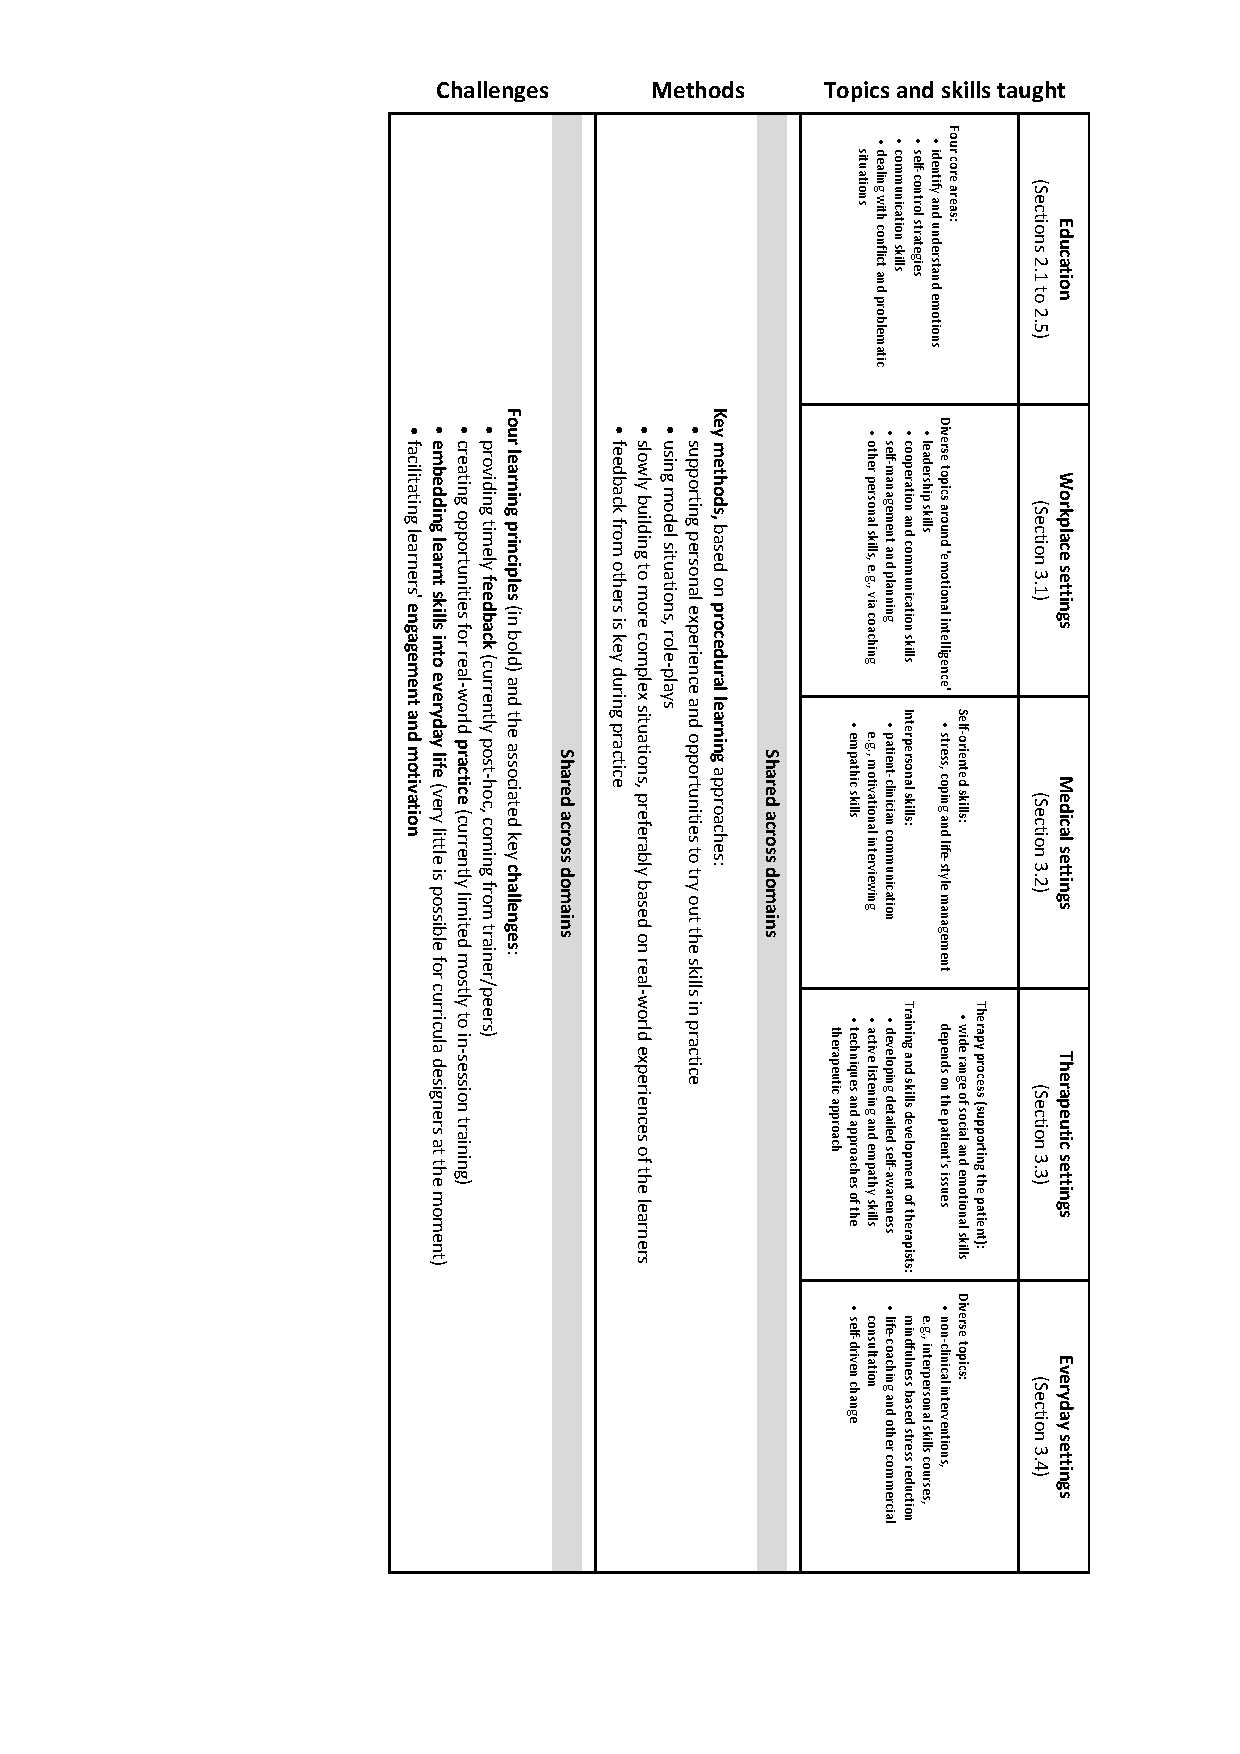
\includegraphics[height=\textheight]{images/SummaryResults}
	\caption{Overview of the key distinctions and similarities}
	\label{fig:SummaryResults}
\end{table}
\fi
%


% }}}
\fi

%{{{ SECTION -  Life skills courses in education 
\section{Life skills courses' contents within education}
\label{sec:SEL}
We start by reviewing the methods, topics and approaches used by SEL curricula in education to teach social and emotional skills. This provides grounding for the next three sections that link the existing SEL practices and challenges to HCI work.
				%  The goal here is to build an overview across the curricula of what gets taught and how, and then use this structure to outline the potential for HCI research. 
%        The overview in this section is deliberately kept quite descriptive and without explicit links to HCI research, although our review process aimed to identify and foreground aspects and challenges relevant to HCI perspective.
%
%We first outline the reasons why we chose SEL for schools as an exemplary domain (section~\ref{sec:reasons}), and describe the literature review methodology (section~\ref{sec:methodology}), before 
        %
%We then present the \emph{methods} used in teaching of social skills in education (section~\ref{sec:methods}),  as well as the key \emph{topics} that  get taught (section~\ref{sec:blocks}), including specific examples from various curricula. 


% {{{ SEL for school
\subsection{SEL in schools as an exemplary domain}
\label{sec:reasons}
%We chose social and emotional learning (SEL) in schools as an examplary domain we review in detail and return to other domains in the next section. %which serves as the basis for a \rephrase{system} of goals, methods and building blocks that encompasses also other domains.
%We outline the reasons for this choice below: 
Social and emotional learning in education is a mature field, with numerous well-researched and evidence-based approaches, and is particularly interesting for a number of reasons:

First, skills taught in school-based curricula are those that have been identified by psychologists and educators as crucial, not only to development in childhood and teenage years, but more importantly as key skills for adult life \cite{Greenberg2010}.  As such, school-based SEL encompasses the core set of skills needed for all domains of life and into adulthood. They also focus on a large span of ages, from kindergarten to high-school education.   %Further, many other life skills domains will often assume some basic level of these skills to have been developed during childhood, and focus then on the deepening of particular subsets of social skills specific to the social and emotional skill needs of the domain.  % as shown in sections below.

Second, SEL has an extensive 20+ years' history of peer-reviewed programs that have already been deployed to tens of millions of pupils. This suggests the potential for considerable real-world impact for any HCI technology implemented as part of a SEL program. For example, \citeN{Durlak2011} reviews 213 program intervention studies encompassing more than 270000 students of all ages, with the interventions conducted over several years. Some studies have their effects tracked for even longer periods of time, as is the case for \citeN{Muennig2009} who recently presented a 37-year follow-up study on the results of a randomized controlled trial of High/Scope Perry Preschool Program conducted in 1962. Moreover, federal programs support further uptake of such curricula in the US \cite{CASEL2013}. 

Third, recent academic reviews have analysed the evidence-base for the effectiveness of SEL programs and find measurable and significant positive effects of SEL in randomised trials, e.g., \cite{Durlak2011,Greenberg2010,Weare2011}. In particular, the social and emotional skills curricula lead to improvements in  academic performance and the taught skills areas. For example, \citeN{Durlak2011} report an average of 11\% improvement in academic performance, and 25\% improvement in social and emotional skills; and there is evidence for positive impacts on many other aspects of behaviour such as mental health \cite{Adi2007a}, violence prevention \cite{Mytton2006,Adi2007b}, conflict resolution \cite{Garrard2007},  and reduction in bullying \cite{Vreeman2007}. %For more detail see e.g., \citeN{Weare2011} who provide a meta-review of 52 reviews in this domain, concluding that the interventions ``had wide-ranging beneficial effects on individual children and young people, on classrooms, families and communities and on an array of mental health, social, emotional and educational outcomes''.

%Despite these achievements, the SEL literature also highlights several problem areas which curricula struggle with---such as the embedding and transfer of learned skills out of SEL training classes and into everyday situations. As we will argue, this suggests, in combination with existing HCI work, that inclusion of digital technology could further enhance and improve the effects and efficiency of curricular training.

%Lastly, the topic also gains increasing political support in the US and Europe, suggesting that social and emotional learning programs for schools might be soon \rephrase{common}. As such, SEL itself provides a novel design space for HCI that could have a strong impact on everyday life and direct real-world applications. 

 %Example of this might be the emphasis on communication skills in medical domains or workplace.


% }}}

        
% {{{ Methodology
\subsection{Literature review methodology}      
\label{sec:methodology}
A large number of systematic reviews of SEL literature already exist, mainly with the focus on meta-analyses of measurable effects and long-term impacts of the curricula (e.g., \cite{Durlak2011,Weare2011,Adi2007a,Greenberg2010,Elbertson2009,Payton2008}). 
%
We build on these and approach the topic with a complementary HCI perspective in mind, aiming to identify the SEL challenges that could be addressed by technology. %To do that, we drew out processes, methods and topics commonly used within curricula, and  the challenges the SEL curricula currently face. 

As such, we analysed the contents of selected curricula, in addition to following references cited by the academic reviews above. This analysis was done by first creating summaries of individual curricula, collating these in mindmaps to draw out related topics, methods and approaches, and finally iteratively identifying the common aspects across curricula and domains. 
%
Given the large number of available curricula for the educational domain, we based our review on a set of curricula selected by the 'Collaboratory for Academic, Social and Emotional Learning' (CASEL)\footnote{\url{http://casel.org/}}. CASEL is a non-profit organisation supporting research and application of social and emotional learning in education, co-founded by leading figures in the academic field. 

In particular, we drew on curricula identified in two CASEL 'guides': the \citeN{CASEL2003} guide reviews 80 SEL programs selected by a rigorous procedure, highlighting 22 of
% P: the first footnote speaks about the programs in general, the second about those that have been highlighted. But I agree it is confusing and should be combined together
 these as particularly well-designed. Each of the 80 programs is described, rated on 15 aspects and linked to academic literature evaluating its effects. The newer version of the guide, \citeN{CASEL2013}, focusses primarily on preschool and elementary school programs, recommending 23 programs.
%\footnote{Out of these, 14 have been already included in the 2003 version, and 9 are new: 4Rs, Competent Kids, Incredible years, MindUP, OpenCircle, Raising healthy children, RULER, Too Good For Violence, and Tools of the Mind.}. 
%
We first systematically analysed the descriptions of all programs in both guides, and continued with more detailed examination of the programs highlighted in either version of the guide (i.e., 34 programs altogether\footnote{Eleven programs selected in CASEL 2013 guide were already selected in the 2003 edition, leaving twelve newly described ones, leading to 34 programs altogether (22+12). \GeraldineTODO{LIST\ THESE\ BY\ NAME\ HERE\ AS\ COMPLETE\ LIST?}}), as well as the academic literature available for each of these programs as referenced in the guides, as long as it was accessible through the libraries of three major universities (yielding 66 academic articles altogether). We also included any course materials and descriptions of the programs that were available on the internet. Finally, we included a number of books on creating SEL curricula in the context of education \cite{Maree2007,Elias1997,Pasi2001,Zins2004,Patrikakou2005}. 





%%Section~\ref{sec:linkDomains}  showing how the identified competencies and methods play out also in the other domains. 
% }}}


% {{{ Teaching methods in SEL for schools

%\vfill ~ \pagebreak
\subsection{Methods for teaching SEL in education -- experiential learning}
\label{sec:methods}

All curricula share an understanding of social and emotional skills as highly complex abilities, drawing also on subconscious processing \cite{Ambady2010,Lieberman2000}. As such, social and emotional skills are based on \emph{procedural} rather than declarative knowledge \cite[p.288]{kruglanski2007social}. Moreover, the key focus of most social and emotional skills is to be able to react appropriately even within `hot' moments, i.e., situations  when the learner is overwhelmed with emotions, and/or the importance of the situation, or just has a very short time to react (e.g., heated conflict). During such moments, the ability of conscious, analytical thought is often diminished \cite{Wyman2010,leDoux1998}, emphasising the need for learning skills that operate on a procedural basis.

%In other words, even if students already have intuitive knowledge on how to react in a social situation, it is problematic to explicitly articulate the processing rules by which they came to these conclusions. Examples of similar dependency on procedural skills can readily be found  in other aspects of our life such as language use, where we know which form in our native language is correct but not necessarily why (``it sounds better''); or in social cognition where people are, for example,  very sensitive to correct proportions of human face, but are not able to explicitly articulate even the most basic ones correctly \cite{Lewicki1987}. 

  

%\subsubsection{Teaching methods used in SEL}
The core of most curricula is a set of SEL focussed, structured classroom lessons \cite{jones2012social}, usually 25-40 minutes long and administered once a week throughout the whole school year (or multiple years). During these lessons, curricula use predominantly active instructional techniques drawing on skill-based and experiential approaches. They employ a wide range of methods such as modeling, role-play, performance feedback, dialoguing, positive reinforcement, vignettes, play and games; as well as other approaches such as portfolios, expressive arts, exhibitions, and group projects -- see Fig~\ref{fig:methods} for an extended list. Through these methods, curricula aim to include extensive examples and opportunities for personal experience and practice, combined with feedback and opportunities for reflection on behaviour and progress. When teaching a complex interpersonal skill such as conflict resolution, curricula break the skill down into less complex sub-skills and focus first on simple model situations. These can be explored by role play (e.g., specific situations such as asking permission to join a game), slowly building up to more complex, but scaffolded situations (e.g., in-class, teacher facilitated resolution of a peer conflict), and eventually to encouraging learners to apply the skills out of the classroom in everyday situations. Repeated practice and extensive feedback from the trainer and peers are critical components in every step of the process in the classroom. 

Once a skill is mastered within the lessons, the key emphasis is then on its \emph{transfer} out of the classroom into everyday contexts to promote maintenance and generalisation \cite{Elias1997,Maree2007,Pasi2001}. This is however one of the current \emph{critical challenges} SEL curricula face, and also one of the main areas where HCI could support SEL (cf. Section~\ref{sec:embedding}). Although curricula highlight the need to support opportunities for the learners to practise their new skills in real life situations outside of the classroom, they have very limited strategies to do so, especially as the scaffolding offered by the teacher in class is no longer available. The current methods used in curricula to support transfer are mainly various activities to increase awareness and remind learners about their skills on the school grounds (e.g., posters around the school), and attempts to enlist the help of their social networks outside of the learning environment such as their parents and other school personnel (e.g., through organising workshops, or sending letters to parents with suggestions how they can reinforce the learning at home). Providing students with activities and exercises to attend to at home or other locations is also common. Overall, however, the curricula struggle to find ways in which to deliver direct support for students outside of the immediate SEL lessons \cite{jones2012social,Maree2007}.  


Curricula are clear that the methods used must be developmentally appropriate for the age of the children, and the skills learned. For example, fantasy play or puppets as role models and curricula protagonists have been very successful methods for younger children (e.g., kindergarten to K-3), who can relate to them easily  \cite{Webster-Stratton2004}. In contrast, group discussions, journal writing and workshop activities are more commonly used with older children and teenagers \cite{dejong1994}. However, specific key methods such as role-playing, modeling, positive reinforcement, and direct and indirect instruction are used throughout in various guises. 
\todolater{Add example from SecondStep pointing to use of videorecordings and workshops for parents ==> highly useful... See \cite[p.88]{Elias1997}.}


%\todo{This is probably not good enough at the minute -- would need one p:aragraph about the parent/community involvement in more detail, if saying that this is an increasing focus or similar blah. Additionally, this combined the embedding into school life, and embedding into everyday, which is probably not what we want?}

\begin{figure}
  \centering
	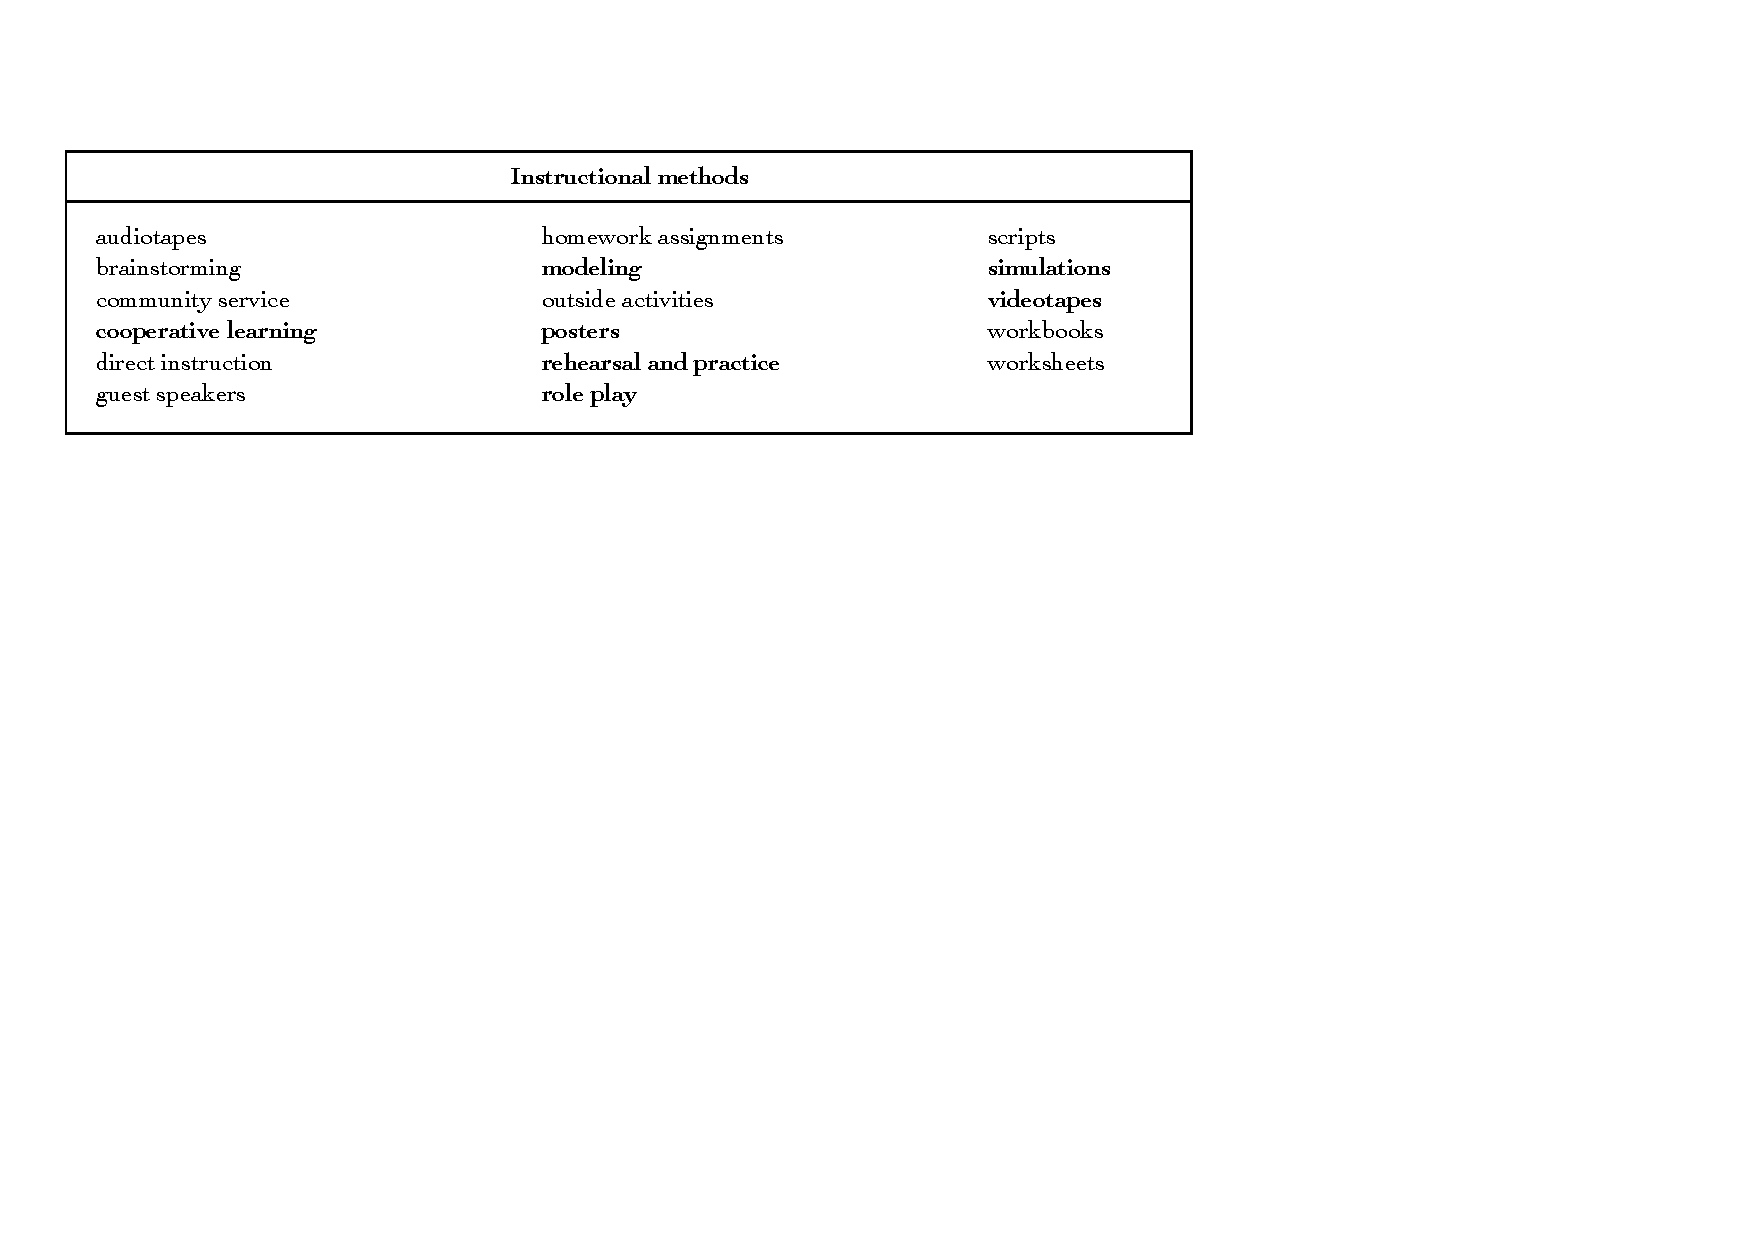
\includegraphics[width=.98\textwidth]{images/Elias-methodsList.pdf}
	\caption{A list of instructional methods used in SEL courses, with those used most widely marked as bold text (modified from \cite[p.109]{Elias1997}).}
	\label{fig:methods}
\end{figure}


%\qq{\cite{Webster-Stratton2004}}{Some strategies that will help young children learn and retain new information include: (1) provide many examples (in different media) of the same concept (videos, role plays, games, cue cards); (2) post cue card pictures in strategic areas to remind children of key concepts (eg, sharing cue card in big block area); (3) role play with puppets (common scenarios such as being teased, rejected, or making a mistake); (4) reenact videotaped scenes; (5) use Dina andWally's detective storybooks to discuss key ideas and generate prosocial solutions; (6) play games designed to practice key concepts (eg, playing “Wally Says”); (7) rehearse skills through activities; (8) give homework to practice skills (ie,Dina's Detective Homework Manual); and (9) send letters to parents asking them to reinforce the skills children learned that week.}

%\qq{\cite{Webster-Stratton2004}}{List of approaches: puppets as models, Live and videotape modeling methods, role-playing and practice games, Helping children learn and remember concepts, Practice activities- coeaching/cueing/reinforcing, integration of affect+coginition+behavioural components, Fantasy play, promoting skills maintenance and generalisation}


% {{{ Common theoretical models
\subsubsection{Common theoretical models}
There is no single theoretical model that would be universally agreed upon by the existing SEL curricula to ground the learning process \cite{Payton2000}. Instead, curricula build on several complementary theories that each have robust evidence of positive effects\footnote{This is similar to psychotherapy domain, where a number of schools co-exist in parallel, each building on different theoretical groundings.}. 
Some of the most prevalent theoretical approaches are: (i) systems theory, which views SEL learning as embedded in the broader community and aims to systematically create a comprehensive climate for teaching SEL not only in the class but also in the school and local communities more broadly; (ii) psychoanalytic theory, which works with how conscious as well as unconscious (unrecognised) emotions shape how we act or learn, and who we are; and (iii) cognitive behavioural theory as a base for primary prevention and the core skill based techniques such as modeling or role-play \cite[p.65]{Maree2007}).

However, despite different theoretical groundings, there is still a considerable overlap among these models in the competencies to be learned (as described in the next section), and a shared set of guidelines on what makes curricula effective. In particular, curricula should take a wide scope both in terms of methods and skills learned, build on a clear theoretical framework, use a comprehensive approach that integrates affective, cognitive and behavioural dimensions, and promote generalisation of skills \cite[p.119]{Elias1997}. Additionally, the literature highlights that piecemeal program efforts, such as one-off workshops, are much less likely to be effective \cite[p.13]{Zins2004} than comprehensive programs.


\todolater{Outline the theoretical background of PATHS, Incredible Years and RULER. What does this mean for technology?}




% }}}

%}}}


% {{{ Topics in SEL
\subsection{Goals of SEL learning}
\label{sec:blocks}



%Whereas the previous section focussed on methods and the general approaches taken to teach social and emotional skills (i.e., "how"), this section focuses on the content, i.e., "what" gets taught. %We aim to outline the commonalities among curricula in terms of the topics taught, the exercices/approaches to do so, and the order in which the topics are learned. % Similarly to above, we draw on thorough perusal of literature describing the twenty-three interventions selected as effective by \citeN{CASEL2013}; as well as other related literature.
%

A set of five core competencies is widely accepted within the educational community \cite{Zins2007,Durlak2011,CASEL2003,CASEL2013} as a good description of the general goals shared by most of the existing curricula, regardless of underlying theories. We quote these competencies and their brief descriptions as per \citeN{Durlak2011}:
%

\begin{figure}
  \centering
	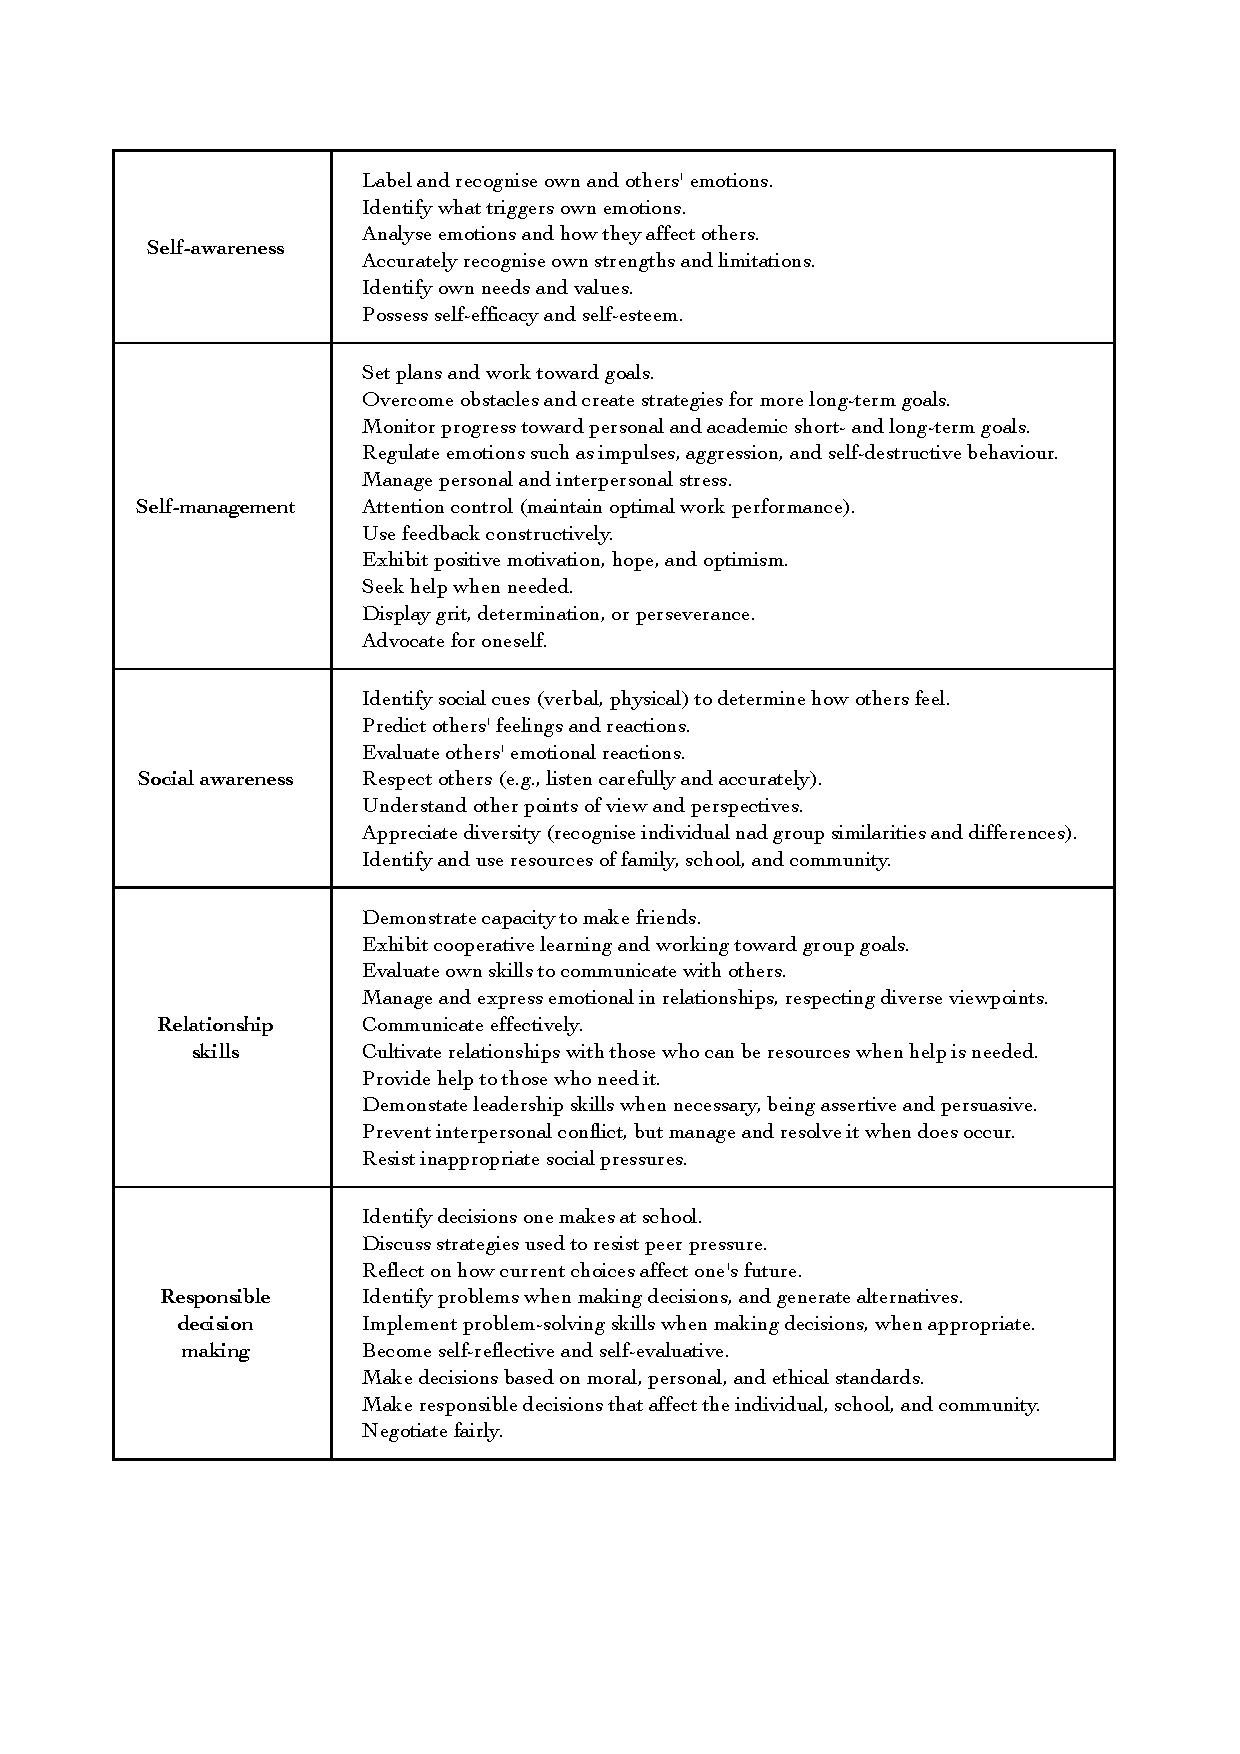
\includegraphics[width=\textwidth]{images/Skills-list.pdf}
	%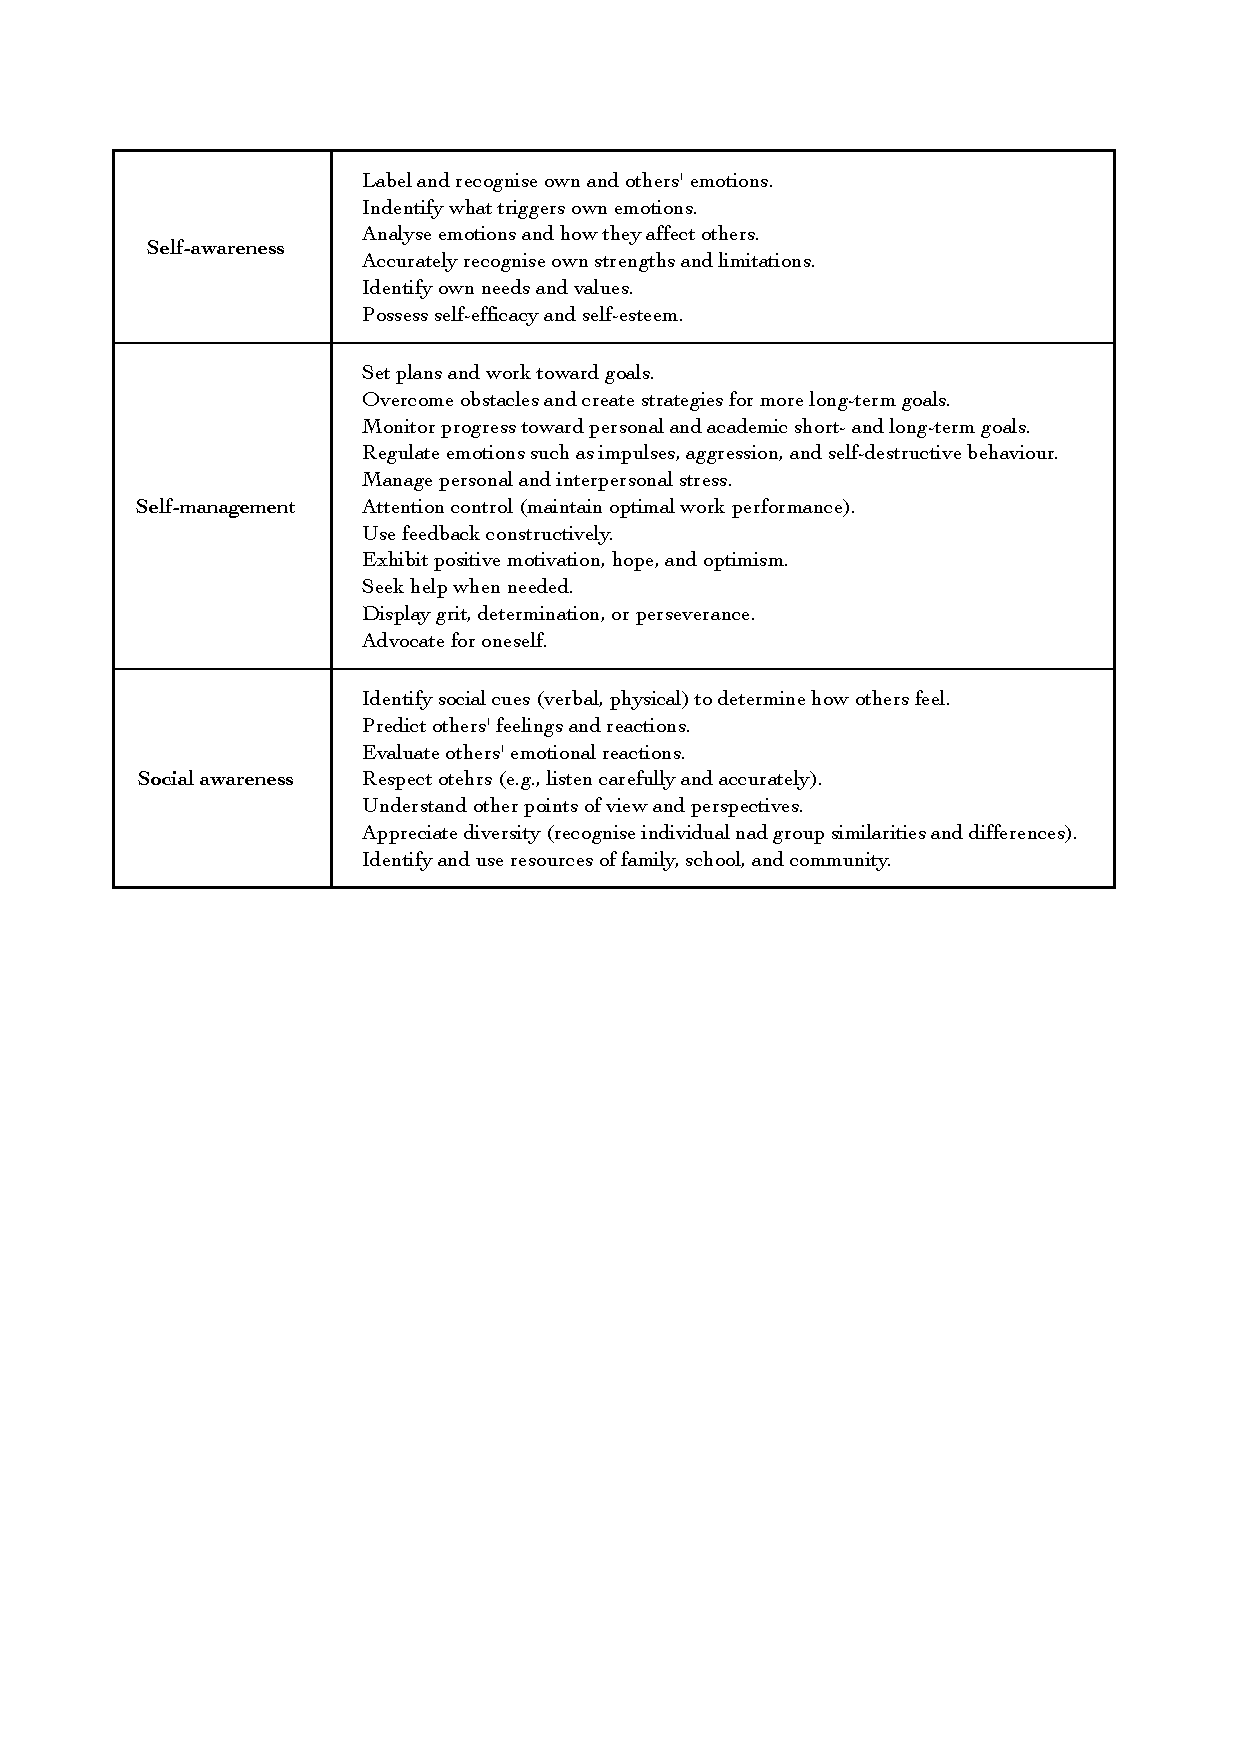
\includegraphics[width=0.85\textwidth]{images/Skills-list1.pdf}
	%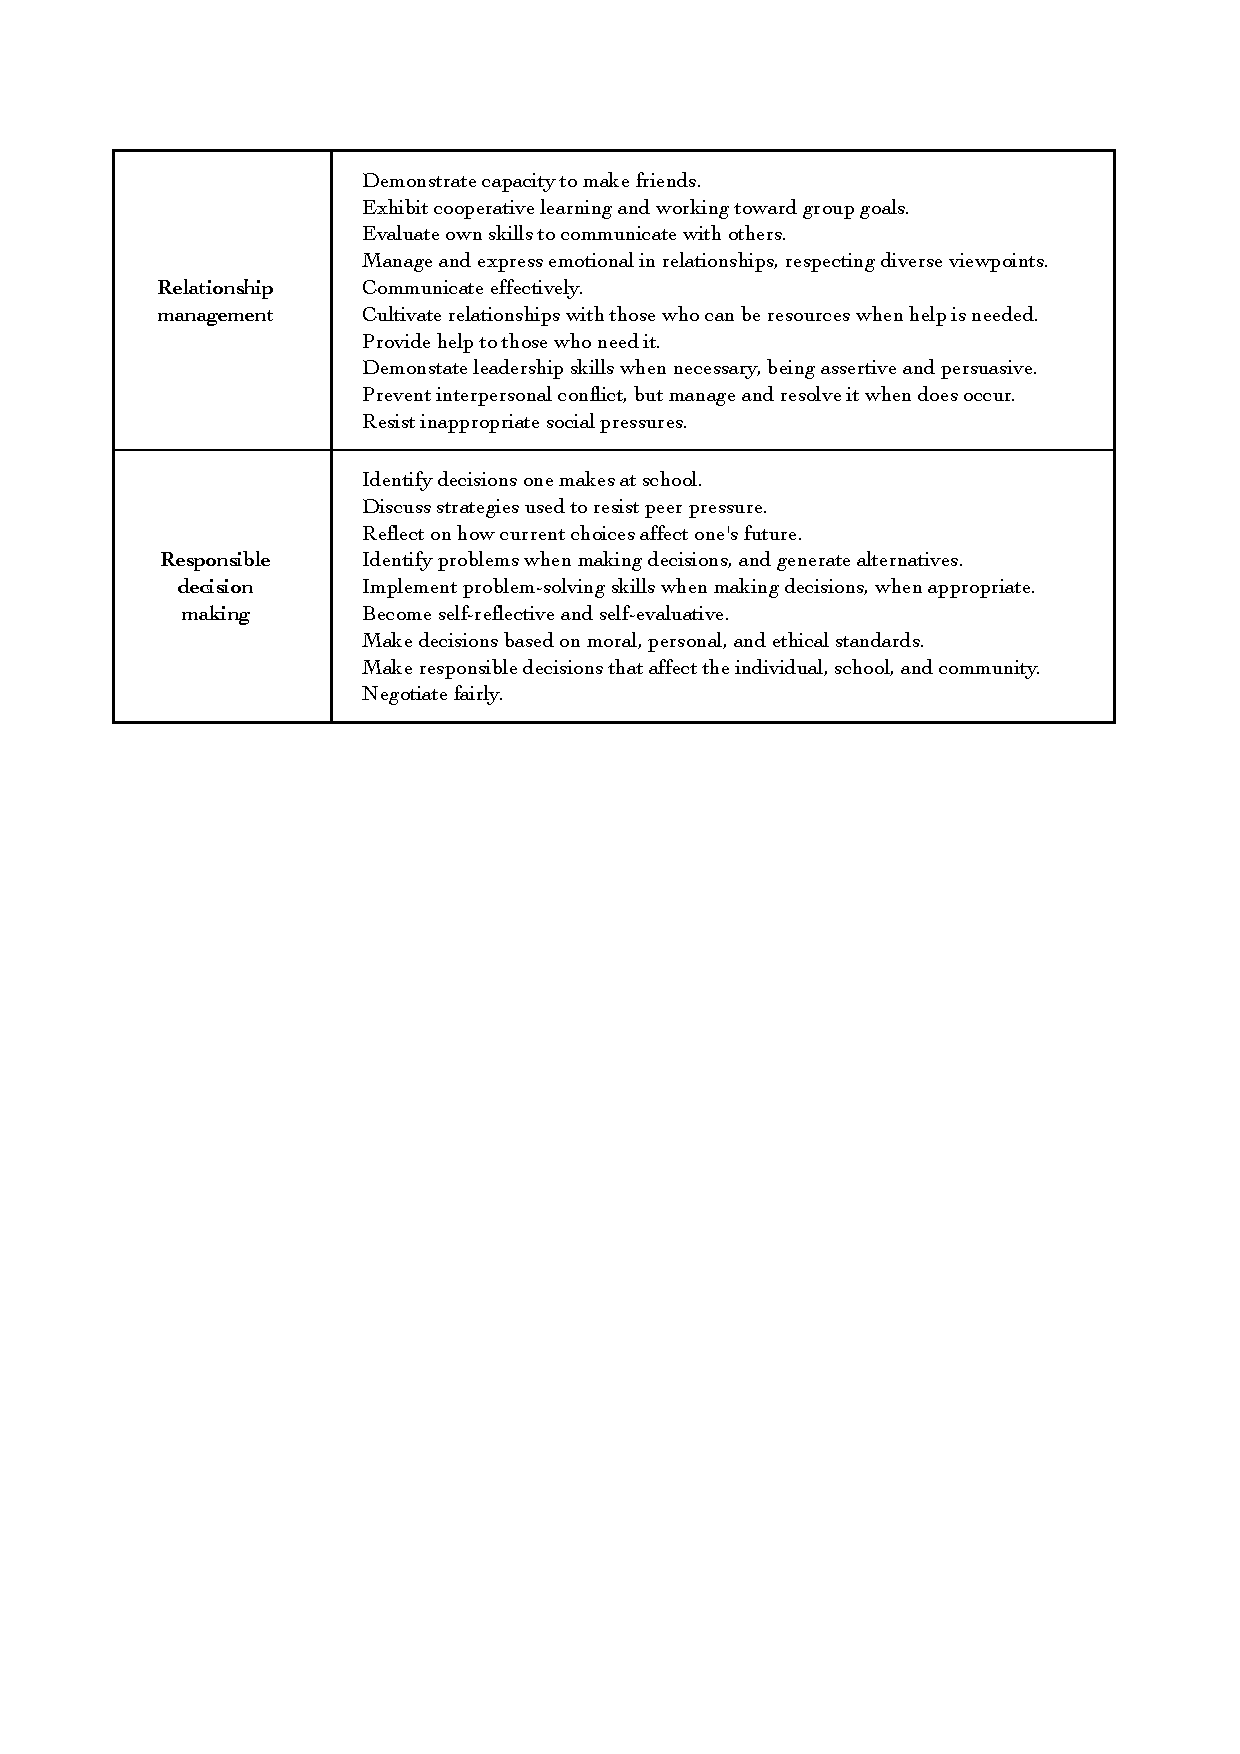
\includegraphics[width=0.85\textwidth]{images/Skills-list2.pdf}
	\caption{Exemplary list of skills relevant to individual competencies \\(from \url{http://www.gtlcenter.org/sel-school})}
	\label{fig:skillsList}
\end{figure}

%\todo{Not a good place for this? .. where does this go?}
%In other words, they provide a good description of the goal state (what SEL aims to achieve), and 
%
% serving as the key overreaching social and emotional skills that SEL curricula teach and promote. 
%


\GeraldineFIXNEW{ GF NOTE: possessive apostrophes below didn't print out in my pdf version}
\begin{itemize}
        \item {\bf Self awareness: }
                        The ability to accurately recognize one's emotions and thoughts and their influence on behavior. This includes accurately assessing one's strengths and limitations and possessing a well-grounded sense of confidence and optimism.
        \item {\bf Self-management: }
                         The ability to regulate one's emotions, thoughts, and behaviors effectively in different situations. This includes managing stress, controlling impulses, motivating oneself, and setting and working toward achieving personal and academic goals.
        \item {\bf Social awareness: }
                         The ability to take the perspective of and empathize with others from diverse backgrounds and cultures, to understand social and ethical norms for behavior, and to recognize family, school, and community resources and supports.
        \item {\bf Relationship skills: }
                        The ability to establish and maintain healthy and rewarding relationships with diverse individuals and groups. This includes communicating clearly, listening actively, cooperating, resisting inappropriate social pressure, negotiating conflict constructively, and seeking and offering help when needed.
        \item {\bf Responsible decision making: }
                        The ability to make constructive and respectful choices about personal behavior and social interactions based on consideration of ethical standards, safety concerns, social norms, the realistic evaluation of consequences of various actions, and the well-being of self and others.
\end{itemize}

However, these core competencies comprise complex, interrelated abilities and it is not possible to teach any of the competencies directly -- see Figure~\ref{fig:skillsList} for examples of the range of skills related to individual competencies. 
Instead, each curricula helps learners progressively develop these competencies, building up from sets of less complex skills. 
%}}}

% {{{ How are competencies taught?
\subsection{How are the competencies taught}
We identified four sets of skills that consistently appear in most of the curricula, and across all age ranges. Our goal is twofold: to provide an initial 'feel' for progression and topics taught in SEL; and to set up explicit examples that can be used in later sections to tie some of the existing HCI research to the approaches presented here.


\begin{enumerate}
        \item identifying and understanding emotions (own and of others);
        \item managing own emotions;
        \item developing communication and relationship skills;
        \item dealing with conflicts and problematic situations.
\end{enumerate}
 % Once mastered, these skills feed into the core competencies described in previous section, as shown at Figure~\ref{fig:strmap}.       
%Although the exact approach, terminology or exercises used by a particular curriculum can differ from others, there is substantial similarity in the focus and emphasis on these sets of skills across the literature.
 
Each set thus subsumes a number of simple situations or skills (e.g., being able to identify becoming angry) and ways to train these (e.g., training learners to notice physical changes in their bodies, such as associated with feeling angry).
Moreover, these topics build on each other in a sequential manner: The ability to identify and understand emotions is a key pre-requisite for managing own emotions (without knowing one's own emotions, one cannot control them), which is in turn needed for keeping relationships (appreciating the perspective of another, not jumping to conclusions) etc. As such, they are taught in the order as shown in Figure~\ref{fig:depfoc}. 
%
We describe each topic in more detail in a respective subsection below, illustrating the descriptions with examples of specific activities from selected curricula.  Figure~\ref{fig:strmap} then maps how the four topics contribute to the core competencies. 




 
\begin{figure}
  \centering
        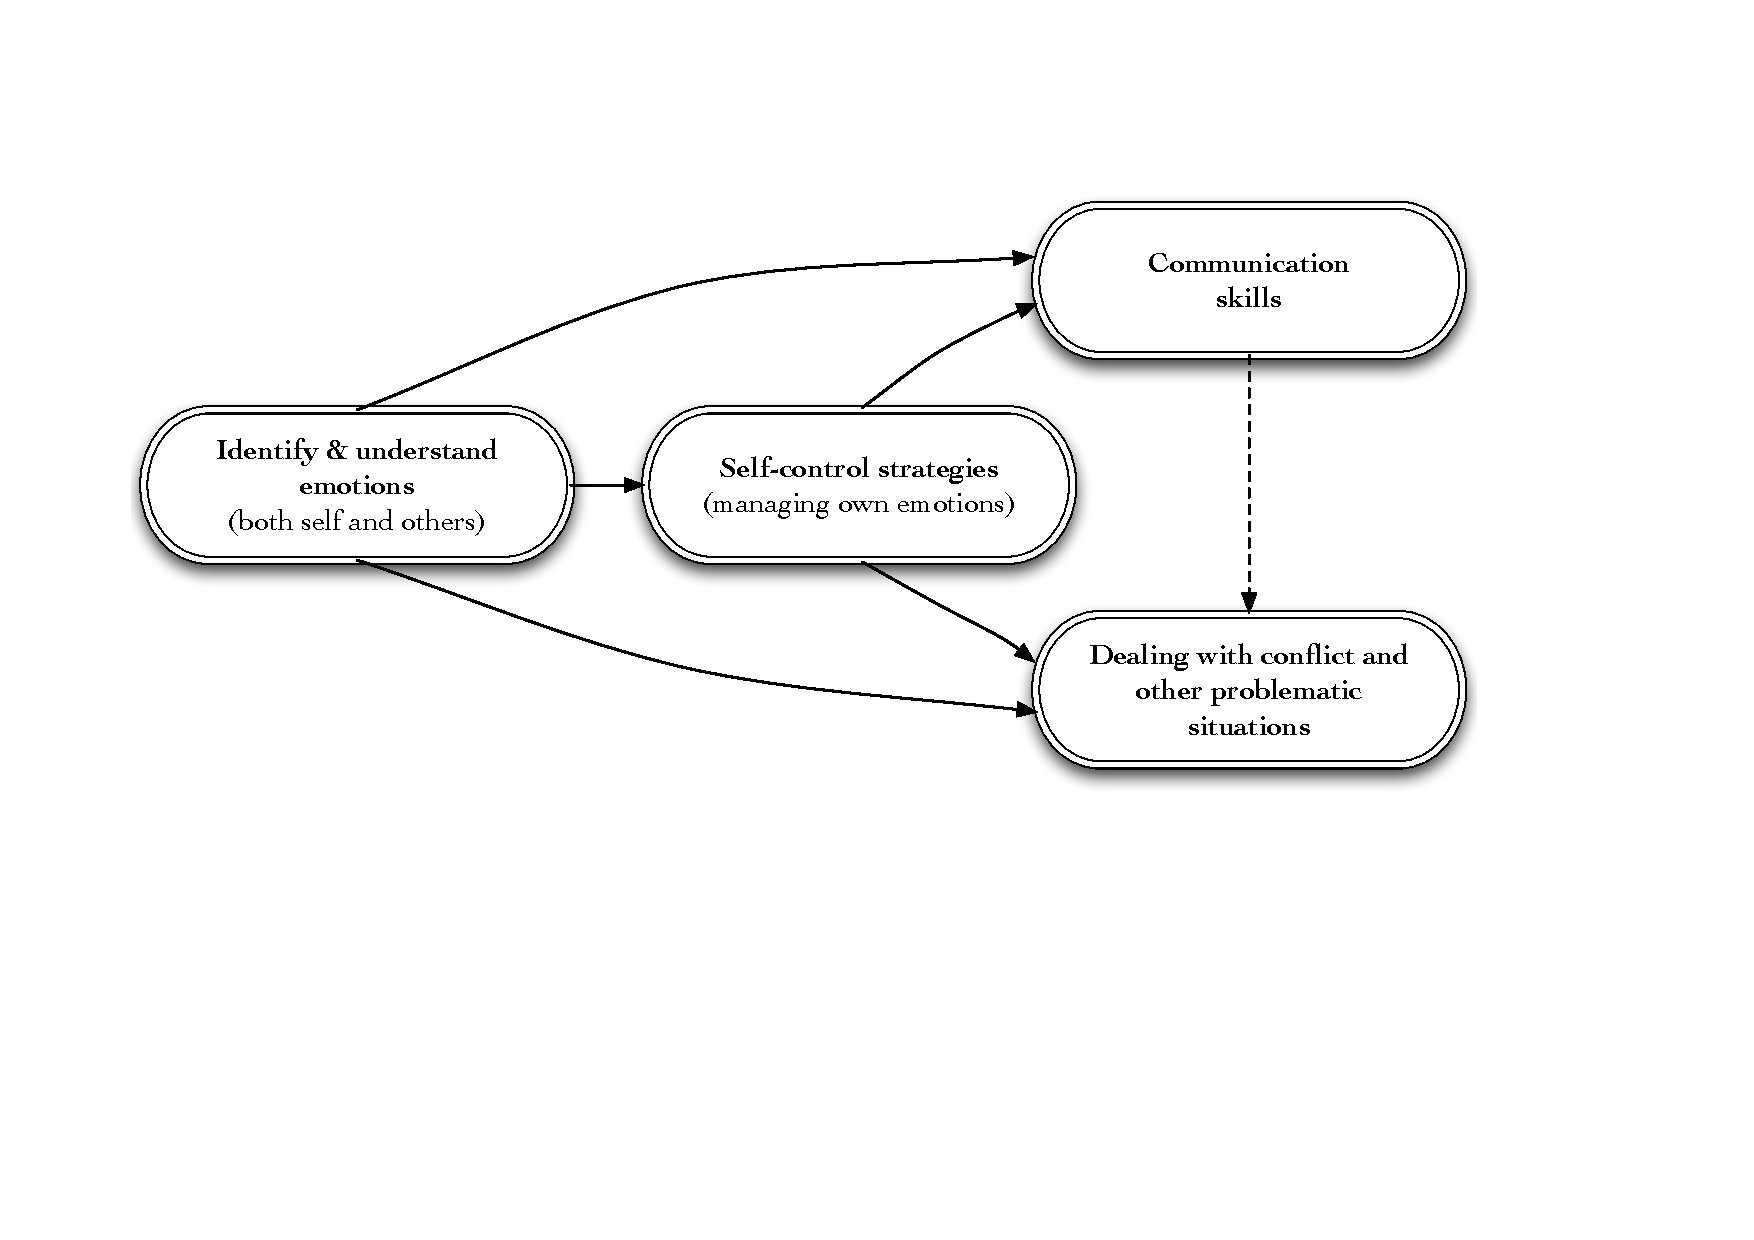
\includegraphics[width=\columnwidth]{images/BuildingBlocks.pdf}
        \caption{Summary of the identified key topics in SEL in education and their dependencies.\GeraldineFIX{G: make clearer that this represents your summary of key topics and dependencied}}
        \label{fig:depfoc}
\end{figure}

\begin{figure}
  \centering
        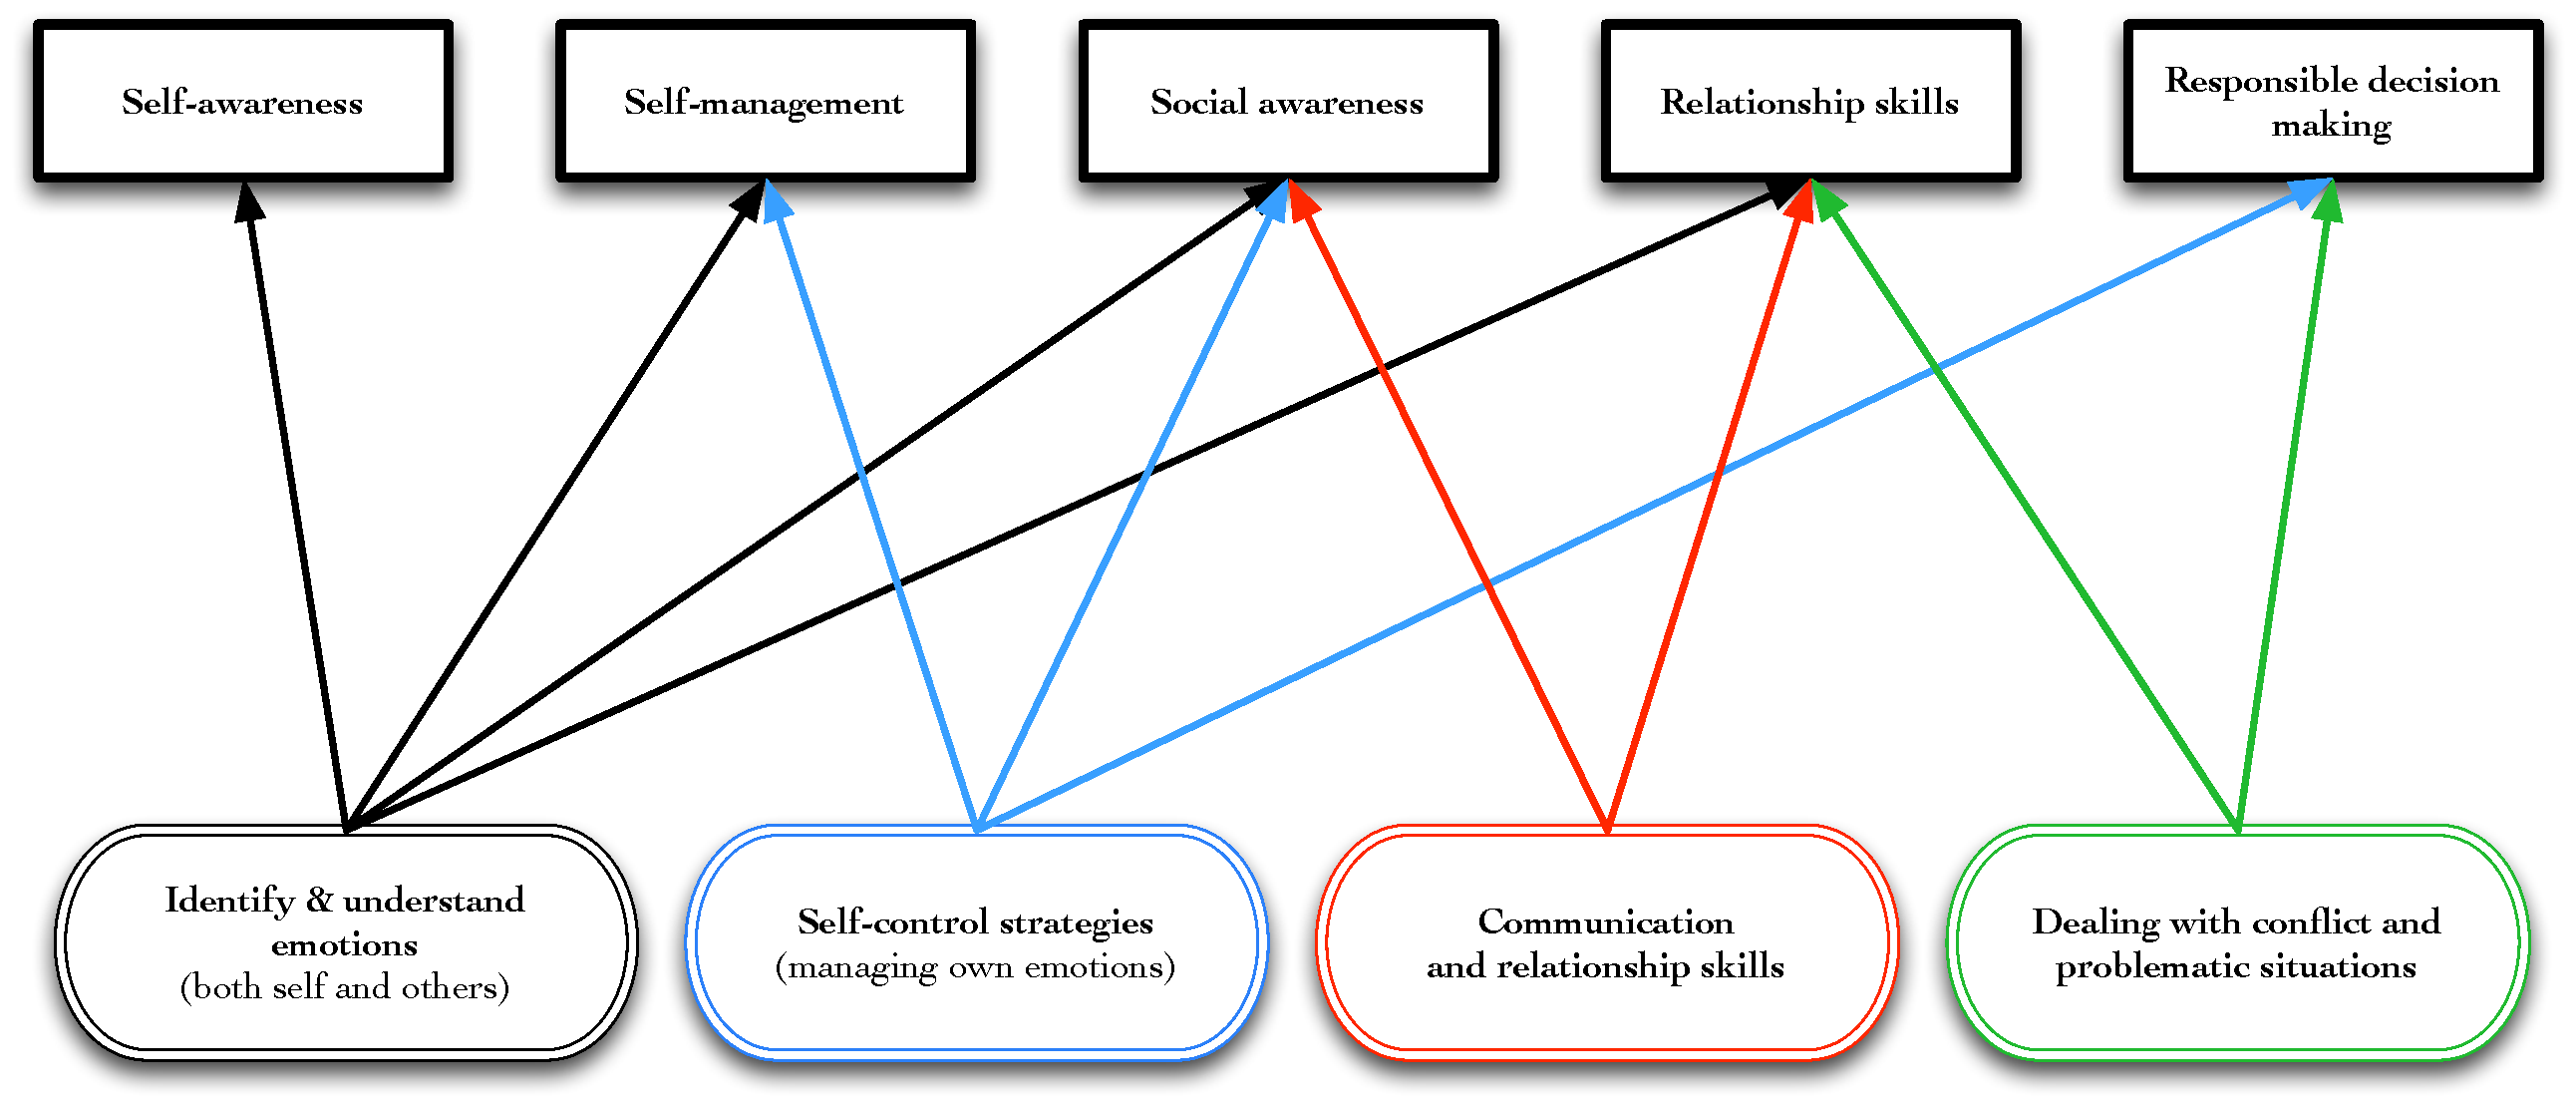
\includegraphics[width=\columnwidth]{images/Blocks-to-competencies.pdf}
        \caption{Mapping of topics to core competencies}
        \label{fig:strmap}
\end{figure}


%\renewcommand{\labelitemi}{$\cdot$}
\subsubsection{Identifying and understanding emotions} 
        %\setlength{\itemsep}{0cm}%

  %\setlength{\parskip}{0cm}%
The ability to identify and understand own and others' emotions is a prerequisite of most other social and emotional skills. A key goal is developing the emotional awareness of learners, which is the ability to differentiate, name and notice subtle changes of emotions. Curricula\footnote{Curricula including content on identifying and understanding emotions are: Caring School Community, I can problem solve, Life Skills Training, PATHS, Peace Works, Quest (Violence Prevention Series), Open Circle, RIPP, Responsive Classroom, Second Step, SOAR, Social Decision Making and Problem Solving Program, 4Rs, Competent Kids, The Incredible Years Series, Michigan Model for Health, MindUP, RULER, Social decision making, Steps to respect, Too Good For Violence. {\bf 21 in total}} aim to train a practice of internal reflection, leading to continuous exploration of how they and others feel. Emphasis is also placed on making the distinction between acknowledging a feeling, and acting upon that feeling/urge. 
\GeraldineFIX{G: all the other subsections list the relevant curricula at the beginning of the section so maybe move the footnote with the list from end of section to here}

In particular, some of the curricula build on language usage, and especially on how use of language affects our thinking processes. Various exercises focus on developing the ability to identify emotions in both oneself and others, helping learners to become more reflexive and self-aware. As an example, the PATHS curriculum  includes physical ``Feeling Faces'' cards, which the child learners use to signal their current emotional state throughout the day \cite{Kam2004,Domitrovich2007}. Similarly,  the RULER curriculum uses popular stories to exemplify particular emotions, and to draw out distinctions among subtle variants of a specific one \cite{Reyes2012}. 
%
Another approach aims to support self-reflection by exploring and understanding how our bodies are affected by experiencing particular emotions. For example, children are helped to recognize their own feelings by checking their bodies and faces for `tight' or relaxed muscles, frowns, smiles, and sensations in other parts of their bodies such as butterflies in their stomachs. Matching the facial expressions and body postures shown on cue cards helps the children to recognize the cues from their own bodies and associate a word with these feelings \cite{Webster-Stratton2004}. 
%               
Emotions of others are explored through the ways in which they affect the tone of voice, body language etc. This is often incorporated as a game, e.g., developing the 'detective skills' to find out how others feel. Repeated   use of similar activities aims to help learners think more often about how they, and others, might feel in various situations. 
\GeraldineFIX{G: do you really mean constant ie no break???}



\subsubsection{Self-control strategies}
        %\setlength{\itemsep}{0cm}%
  %\setlength{\parskip}{0cm}%
Self control and management of own emotions is a key aspect of many curricula\footnote{Life Skills Training, Lion's Quest, PATHS, Peace Works, Productive Conflict Resolution Program , Quest (Violence Prevention Series), Open Circle, RCCP, RIPP, Responsive Classroom, Second Step, SOAR, Social Decision Making and Problem Solving Program, Teenage Health teaching Modules, 4Rs, Al's Pals, Competent Kids, The Incredible Years Series, MindUP, Positive Action, RULER, Steps to respect, Too Good For Violence. {\bf 24 in total}} and the techniques used to develop self control build on emotional awareness.%, aiming to teach strategies for managing strong emotions once they are recognised. 

Various strategies and exercises aim to help participants to relax and/or calm down once a strong feeling is recognised. These are often based on various physical exercises such as muscle stretching and deep breathing techniques. Other strategies draw on verbal labelling, building on psychology and neuroscience findings showing that the act of consciously labelling an emotion by name (rather than ``just'' being aware of it) facilitates higher cognitive control over the emotional state \cite{Greenberg2006,Reyes2012}. Exercises training explicit acknowledgement of emotions, as well as thinking about what could be their cause, are often used. 
Specific strategies for anger management are particularly common, often combining both verbal labelling and physical relaxation exercises. An example is the ``Turtle technique'' \cite{Robin1976}, which is still used in a number of curricula (e.g., Incredible Years or PATHS). In this technique, children are taught to ``withdraw into their shell'' (by pulling their arms and legs close their body and closing their eyes) at specified occasions such as when they feel increasingly angry. This is followed by a relaxation phase, where specific muscle groups are tensed and released. Once this technique is mastered, children discuss appropriate alternative strategies for dealing with stressful situations, now that they are able to consciously reflect and react to them. 
\todolater{For older children, self-control exercises focus on supporting personal management more broadly, such as promoting goal setting, self-motivation and grit.}
%\todo{Add a sentense around older students -- self-control as important to support motivation and grit}

\subsubsection{Communication skills}%Facilitating positive relationships},
Another set of activities focuses on building good communication skills and supporting positive interactions with others\footnote{While implicit in many others, this aspect is explicitly highlighted within the following curricula: Michigan Model for Comprehensive School Health Education, Peace  Works, Open Circle, RCCP, Responsive Classroom, Second Step, SOAR, Tribes, Al's Pals, The Incredible Years Series, MindUP, Positive Action, Steps to respect curricula. {\bf 13 in total.}}. The skills taught here are aimed at supporting respectful empathic communication and thus implicitly facilitating friendship relationships, and an ability to collaborate and avoid conflicts that could otherwise occur through misunderstanding. 

The emphasis is on teaching active listening, which is then used to facilitate teaching empathy. Other teaching strategies also focus on training of specific communication skills (e.g., giving and accepting compliments).
Exercises can include games to: induce collaborative activities; practise active listening, e.g., through listening to someone telling a story and then trying to rephrase it with as many details as possible; and disagree respectfully. These can include ways to subtly reframe a message into a form which is not threatening, such as in \citeN{ABER1998} where students are taught to acknowledge the potential mismatch between their and the other's perception of the situation (e.g., preferably saying "It seems to me you are not listening now.", rather than ``Why aren't you listening to me!'').%\todo{Stronger connection to building relationships needed?}

\subsubsection{Dealing with conflicts and problematic situations} 
Problem solving strategies and conflict management are the final topics of most curricula\footnote{Michigan Model for Comprehensive School health Education, PATHS, Peace Works, Productive Conflict Resolution Program, Quest (Violence Prevention Series), Open Circle, RCCP, RIPP, Responsive Classroom, Second Step, SOAR, Social Decision Making and Problem Solving Program, Tribes, 4Rs, Al's Pals, I Can Problem Solve, Competent Kids, The Incredible Years Series, Positive Action, Social decision making, Steps to respect, Too Good For Violence. {\bf 22 in total}}.  Violence prevention is commonly an important additional goal, as many of these curricula are designed  for all schools, including those with a high prevalence of aggression and weapon use. 


Students are often taught a particular structure of reacting to a problematic situation or a conflict.
%
A key approach is to help students process the situation on a cognitive level, despite the fact that conflicts tend to ignite strong emotions. For example, the PATHS curriculum includes a ``semaphore'', where the sequence of red-yellow-green indicates a "stop-think-proceed" process \cite{Kam2004,Domitrovich2007}. Such structured sequences always include and emphasise a goal setting and evaluation phase. Moreover, curricula aim to teach children and teenagers to recognise which conflicts might have arisen from misunderstanding, with perspective taking exercises forming the core approach. An example is exploring win-win negotiation (e.g., in RCCP) in a workshop format and providing suggested sequences for steps to take during disagreements (e.g., in Incredible Years).



% }}}

% {{{ Differences across grades
\subsubsection{Differences across grades}
\label{sec:ageDiff}
Curricula exercises are designed for specific grades/age levels, keeping in mind the developmental changes in abilities of the learners. For example, curricula for K1 students can aim to help the learners label and identify basic emotions such as fear or happiness, K4 students might focus on more complex emotions such as jealousy or embarrassment, and high-school students would be taught to draw on their more nuanced self-awareness to motivate goal-setting and critically assess their behaviour. Curricula also particularly highlight the increasing integration of cognitive, emotional and behavioural aspects that can be expected of students as they grow older. See, e.g., \citeN[p.133-138]{Elias1997} for more detailed information on the progression and detailed changes in skills foci. 

% }}}





%}}}
%}}}

% {{{ SECTION -  Supporting SEL with technology
\section{SEL challenges and opportunities for technology support}
\label{sec:HCIsupport}

Despite the success of curricula in promoting learning of social and emotional skills to some extent (cf. Section~\ref{sec:reasons}), the review of SEL literature also highlights areas where novel approaches are needed, or further improvements are possible. In the rest of this section, we outline three such exemplary topics---embedding of skills into everyday settings, promoting reflection, and providing mixed spaces for practice. Our choice of highlighting these particular areas was motivated by the extent of related HCI work that exists for each of these. This allows us to exemplify the potential for collaboration of HCI and SEL, and specifically point to existing HCI work that suggests how incorporating digital technology may help address crucial needs in, as well as open new opportunities for, SEL in education. 


%The review of SEL have clearly outlined the fundamental role of experiential learning in development of social and emotional skills.

%We now highlight embedding as the key aspect through which digital technology may address a crucial need within SEL learning. Moreover, we also highlight promoting reflective abilities and mixed learning spaces to support further practice as two other areas where, based on existing work in HCI, we argue use of digital technology could bring novel opportunities to support and enhance current learning.

\GeraldineFIXNEW{GF NOTE: do you need to make it clearer what the challenges are and then also be clearer that you are structuring this discussion more by relevant work in HCI than the SEL categories you pulled out earlier? Otherwise raises questions about why these categories for this discussion???}


%Note: 
%We choose a specific format for this session, we always outline a particular challenge/issue existing in the SEL learning, using these to provide exemplary ideas for possible technology support. These are however not intended to provide the solutions (as any solution would need to be tailored to the SEL program, age of children etc.), only to illustrate the possible areas where technology could be useful, and which could be designed for. 
%
%Especially for the embedding part, many of the proposed use-cases revolve around novel sensor and other tracking aspects (SSP). While the current state-of-art might not be robust and reliable enough to be directly deployable in SEL settings yet, we argue that existing studies suggest opportunities for these to be so in future; in addition such use-cases can serve as benchmarks for viability of the setting and thus provide important guidance for future development.




% {{{ Embedding
\subsection{Embedding of learnt skills into other settings}
\label{sec:embedding}
We start with what the SEL literature highlights as one of the key issues with existing SEL curricula -- i.e., the lack of support for transfer and 'embedding' of the skills students learn in SEL classes into their other real-world interactions, be that still within school (other classes, playground) or everyday behaviour within family and peer groups \cite{Maree2007,jones2012social,Patrikakou2005,Elias1997}. 
%
While such transfer of learned skills is the ultimate goal of all curricula, the current approaches are limited in scope and effectiveness. This leaves teachers (and curricula designers) struggling to directly influence the embedding of skills outside of the SEL learning sessions, be that in other classes, or outside of school completely.
%
For example, \citeN{jones2012social} summarise the situation as follows: \qqq{Perhaps most important, and often overlooked, is the fact that SEL programs are rarely integrated into classrooms and schools in ways that are meaningful, sustained, and embedded in the day-to-day interactions of students, educators, and school staff [\dots] Most SEL programs focus solely or primarily on what goes on in the classroom, but SEL skills are also needed on playgrounds, in lunchrooms, in hallways and bathrooms -- in short, everywhere. These non-classroom contexts provide vital opportunities for students to practice their SEL skills.}
%
\citeN[p.70-71]{Maree2007} further highlight the critical role of adults, both in and out of school, in the success of SEL training for students: \qqq{Many SEL efforts fail because long-term, coordinated plans and school-home partnerships are not developed. [\dots] [T]he efforts of school-based practice falter because educators are not committed to being ongoing, vital SEL role models. SEL involves not just the students in schools but also the adults in their lives: teachers, parents and the wider community. If these adults lack social and emotional competency, children will quickly notice the discrepancy between behaviors that the adults advocate for children and the actions that the adults take themselves.}


%As such transfer of learned skills from SEL-specific class exercises to other activities in and out of school is a clear key challenge for the existing curricula [ref,ref].

We argue that digital technology could support these efforts in at least two ways: first, by extending the learning support and scaffolding for learners beyond the SEL lessons, e.g., utilising mobile and sensor based technology; second, through facilitating a wider community of support for learning of social skills, including the involvement of parents and teachers -- not only by connecting them to the learning content in the classroom, but also enabling vicarious learning so that they develop their own social and emotional skills. We outline each in more detail below.

% {{{ Supporting learners directly
\subsubsection{Supporting the learners  -- Transitioning the skills out of the SEL lessons}
\label{sec:Embedding-learners} ~ \\
When SEL skills are to be transferred beyond the SEL classroom lessons, the learners can no longer take the advantage of the direct scaffolding normally provided by the teacher and the lesson structure. This brings several difficulties for the learners to reinforce and apply their skills outside of direct SEL training. We particularly highlight the difficulties with (i) identifying moments when the newly learnt social and emotional skills could applicable, (ii) the lack of scaffolding and support to do so, and (iii) the need for 'space' to reflect and learn from the experience afterwards. 

%We start by discussing the specific setting around SEL in/out of classroom, and the  \todo{Can we fit the in class/out of class dimension into here directly? Or at least make obvious that we talk about specific, fixed location and a set of SEL learning that can be supported, and the ability to 'ask' students to volunteer and use particular gatgets (as opposed to random people with a mobile phone at a random location) -- should we have a little section on setting affordances upfront? }
%\todo{Highlight this aims to support a novel informational overlay over existing real-world interactions that provides scaffolding for re-inforcement and transfer or learned skills in other contexts. As such, will bring serious challenges for HCI research in terms of robustness etc.; however school and still learning settings might ameliorate some when compared to completely in the wild studies as described above. }

\paragraph{Identification of teachable moments}
When interacting during breaks, other classes, or outside of school completely, the learners encounter many occasions that are relevant to their SEL skills learning. However, the learners may not recognise such opportunities and instead revert to previous, negative behaviours (e.g., an angry outburst rather than a self-controlled reaction), especially if emotions are strong and no external guidance is available \cite[p. 56]{Elias1997}.  In such situations, it is thus not only difficult for the learner to apply the skills they have learned, but even to perceive these as such 'teachable moments'. This is one of the key differences to the SEL class setting, where it is the role of the teacher to facilitate and point out situations in which students could use their (new) SEL skills, and reinforcing them if they do. 
%
Curricula designers therefore suggest that all school personnel should \inqq{play an important role in actively encouraging and reinforcing the use of skills and attitudes they see displayed} (e.g., \cite[p. 56]{Elias1997}). This however requires the (possibly untrained) teachers to constantly strengthen and actively encourage use of SEL skills in addition to all their other duties. More critically, there is little opportunity for supporting the learners when the teaching staff are not around (and thus also making the students fully dependent on external guidance e.g., from parents). 

This points to the benefits of (and the need for) technology that could support the learners themselves in noticing and reacting to the relevant situations. For example, learning self-control is one of the key aspects of SEL; it relies strongly on identifying a problematic situation and then to calm down before it is 'too late' and emotions are already running high. One opportunity for technology in this setting can draw on the maturing HCI research on in-the-wild stress detection drawing on physiological data or speech prosody, e.g., \cite{Hernandez2011,Poh2010,Pina2014,Zeng2009,Ertin2011}. We envision that such data could be used to support the learners in becoming aware of their heightened arousal (e.g., through a private tactile reminder such as FitBit wrist vibration), which can serve as a cue to start the self-calming/self-control mechanisms taught in class. Earlier research in HCI suggests that providing such on-going subtle cues for facilitating awareness, and triggers that remind users to attend to intended activities, can be useful to help users modify their existing behaviours \cite{Consolvo2009,Obermair2008}. Moreover, SEL designers have deep understanding of how best to work with such cues and triggers once these are identified. An example of initial work in this direction is \citeN{Pina2014}, who designed a system for parents of ADHD children, delivering in-the-moment cues and strategies to manage stress during everyday activities.  Overall, the initial studies point to the potential of such technologies, but also point to many practical issues to be addressed, including whether such systems are robust and precise enough for immediate inclusion into the SEL curricula, and how could these be best embedded in the existing programs to most appropriately exploit this potential. 

\todolater{???Other similar opportunities for technology could be in supporting other learned topics such as prompting awareness of own emotions, }


%Similarly, this brings opportunities for novel tracking made available by recent advances in Social Signal Processing (such as detection of shouting or anger from speech intonation and intensity \cite{Vinciarelli2012}), should it prove robust enough for 

%\rephrase{Alternatively, technologies helping students identify learning moments could leaving detection on the learner but supporting better focus -- e.g,  through journalling and other reminder methods, digital technology has been shown to support the users paying more attention to activities of interest -- think of something like the noticing button, or young kids asked to take pictures of students engaging in 'supported' behaviours (e.g., lending toys, playing together ...)}




\paragraph{Scaffolding and structure to support training of skills}
Learning of skills is scaffolded in many ways within SEL training sessions:  (i) the scaffolding inherent in the activity itself, such as a prepared scenario for a role play that highlights a particular aspect to focus on; (ii) the teachers' presence and input into the activity, such as prompts guiding the development of the role-play, and feedback to students on their behaviour; and (iii) also the fact that this is a SEL training session, which brings a particular set of foci for the students including the explicit attention paid to SEL skills development. However, much of this scaffolding disappears outside of the SEL learning, even if the situation is still within a class setting (e.g., during a lesson in a different subject). 

% , but similarly in other curricula. Schools currently deploy posters around the school with the aim to support students' ability to remember and use these in the important teachable moments. However, these do not seem to be very efficient \ref{Cohen2006}.

This points to the opportunities for technology to provide just-in-time prompts, reminders and structuring, e.g.,  through mobile devices, to support the scaffolding of activities and help learners focus attention on SEL skills in play. 
%
Examples of such direct scaffolding methods that can be useful out of SEL classes include problem solving strategies such as the 'stop-think-proceed' semaphore in the PATHS program and the sequence of steps to resolve disagreements in the RCCP program, where each person is invited to share their perspective on the situation in turn. Within HCI, several projects have explored technology support for similar structuring as part of autism therapies. For example, the MOSOCO project \cite{Escobedo2012,Tentori2010} exemplifies how mobile phones can help children on the autistic spectrum structure, but also their neuro-typical peers, to structure and practise their social skills outside of lessons, and how the system can help elicit feedback from their peers. Similarly HygieneHelper \cite{Hayes2013} and SocialMirror \cite{Hong2012} help scaffold everyday activities for people with autism. While the social aspects supported in these systems are relatively basic when compared to the full range of skills taught as part of SEL, they none-the-less raise the question about whether similar approaches might be possible for more complex behaviours. Initial work has, for example, explored the use of similar technology to deliver personalised strategies for coping with stress in everyday life for a general population \cite{Paredes2014}; and \citeN{Mamykina2008} designed MAHI, a mobile-based scaffolding system for newly diagnosed diabetes patients that extends the in-class lessons by facilitating participants' ability to track, reflect on and analyse their everyday experiences with diabetes, leading to improved feeling of control over the disease.


Another example for possible scaffolding through technology is the crucial importance that the initial phases in all curricula place on the ability to be aware, acknowledge and importantly also label emotional experiences over time. We saw curricula using methods such as FaceCards while in class (PATHS); or even structuring the whole curriculum around this skill (RULER). The power of mobile technology to prompt and collect such emotional reflection on-the-go presents opportunities to further extend such emotional awareness into other settings; and a number of projects have already explored related techniques in various contexts in existing HCI work. In one such example, \citeN{Matthews2011} developed a ubiquitous application to support emotional awareness training  for psychotherapy clients, using mobile phones to elicit and support reflection on current emotional state regularly over the course of the day. As part of other initial work, \citeN{Munson2010} integrated the Three Good Things, a well-known positive psychology intervention, into a social networking site, meshing it with users' daily habits around these sites, and thus facilitating social and emotional awareness through technology. 
%
Although these projects did not focus on the specifics of emotional training in SEL (e.g., distinguishing between a particular set of emotions depending on age, or exploring the set of activities that led to that particular state), the design mechanisms behind these applications could likely well be transferable to the SEL settings. 
% The systems supporting reflection have mostly been developed with real-world use in mind (\cite{McDuff2012,Balaam2011,Stahl2008,Moraveji2011}). 

\paragraph{Support opportunities to stop-and-learn from experience}
Providing opportunities for post-hoc reflection on one's own behaviour is a crucial part of experiential learning, helping learners make sense of their experiences
% GF: POST HOC REFLECTION --- vs reflection discussions in 3.2?
% GF: ALSO --- more to be made of the distinction between (or opportunity for both) reflection in the moment of action/interaction and later reflection or reflection outside of the class that can then also be brought back to the SEL classroom
 \cite{Moon1999,Cohen2001}. As such, SEL class-based activities include explicit time to reflect on own experiences, e.g., in the form of a debriefing or discussion after a role play. However, such post-hoc reflection might be difficult for situations outside of the SEL training scenarios, where the teachable moment is intertwined with other continuing activities that may prevent immediate reflection (e.g., resolving a conflict around what game to play during recess, which once finished, leads into the game right away). Students may end up not reflecting at all, or, if they do, find it difficult to recall the situation and their own reactions well (e.g., \cite[p. 55]{Pasi2001}).

While only limited work exists in HCI around supporting such processes for social and emotional learning specifically, the growing focus in HCI on supporting reminiscence and reflection in other contexts suggests ways in which technology could support learners in collecting traces of aspects of their experiences to ground later reflection, e.g., \cite{Fleck2009,Marcu2012,Sanches2010,McDuff2012}.  
%; see Section~\ref{sec:feedback} for more details.  
%
SEL sessions in current curricula already include discussions around SEL-related issues that students experienced in the meantime\footnote{For example, the teachers following the PATHS curricula keep a ``Problem box'' on their table. During the day, students experiencing problems can write them down and place the note into the box. The resulting issues are used once or twice a week to seed problem-solving meetings \cite{Kam2004}.} and such collected data could be incorporated to ground the discussion and learning. 
%
While we provide a more detailed discussion of other HCI work around supporting reflection in Section ~\ref{sec:feedback}, one direct example of using such recorded data to support SEL learning comes from the literature around Video Interaction Guidance (VIG) framework. A number of studies provides evidence of how guided, post-hoc reflection of micro-moments, selected from video clips of everyday activities, can promote social skills learning (see e.g., \cite{Kennedy2011} for a summary). While primarily developed to support parents of children with behavioural issues, it has since been applied to promote learning for various groups, such as teachers, psychologists, and counsellors,  and might be a valuable addition to existing curricula. Importantly, novel systems could draw on and extend the VIG framework to support the learners themselves in capturing such micro-moments for their later reflection and analysis.   

%In one such example, \citeN{Fleck2009} explored the use of SenseCam to support reflection by teachers around their teaching style and abilities. The authors report how the resulting images, automatically captured during the lesson, were used to ground the reflection process by supporting teachers to return to their experiences, and promoting a rich understanding of their own and other's activities. Similarly, \citeN{Marcu2012} provided wearable cameras to children with autism, promoting sharing of experiences around the resulting images and their social engagement with their parents and therapists. Moreover, HCI exploration of systems aimed to trigger reflection on emotional aspects of everyday life might also suggest new approaches to support SEL relevant learning. For example, AffectiveDiary combined biometric data, movement and mobile phone use to present the users with intriguing ambiguous visualisations, facilitating sense making and reflection on their everyday activities \cite{Stahl2008}. Other work looked at using collected data to promote reflection around stress \cite{Sanches2010} or work activities (e.g., \cite{McDuff2012}).
%
%





%  POSSIBLE ADDITIONS 
%
%We expect that the ability to trigger SenseCam-like images as based on social signals tracking algorithms (e.g., stress level) could open other interesting options for future work.  
%
%Learners could also benefit having the ability selectively record aspects of situations for future analysis. For example, \citeN{Hayes2008} automated recording that saves only 5 minutes before a button press, to make sure interesting aspects are not missed, but also to address privacy issues. While this is currently in control of teachers, similar mechanisms could be made to work for the students themselves, empowering them to be better able to collect data they need for their reflection and learning. \rephrase{Although this raises obvious privacy and ethical considerations, a potential benefit of designing such technology as part of learning contexts within schools environment is that this would allow for specific constrains and safeguard regarding the use to be put in place and enforced by the teaching staff.} 



%Video Interaction Guidance framework \cite{Kennedy2011} draws on video-recordings of everyday  activities social skills learning through guided reflection on selected aspects of the interaction. A substantial evidence-based 


% }}}


% {{{ Social support
\subsubsection{Social support -- community building} 
\label{sec:Embedding-social}
~ \\
Literature around SEL curricula highlights the importance of a supportive atmosphere, not only in the school but also at home, which is crucial to successful learning \cite{Maree2007,Patrikakou2005,Pasi2001}.  Support from the parents as well as learners' peers is thus needed, but difficult to promote in the existing curricula. Although there is only limited work in HCI that addresses supporting such links between school and home, we argue below that the extensive knowledge HCI has gained in other settings around promoting the development of support networks \cite{Skeels2010,Massimi2013,Barak2008} and local communities \cite{Ganglbauer2014,Lewis2012,Lopez2013,Massung2013} makes it plausible that HCI will be able to contribute here as well.

\paragraph{Peer support}
Interaction with, and perceived support from, peers are both crucial for school-age learners, especially when they are in their teenage years. Systems utilising the learners' broader social network could help motivate and engage participants to keep up with their SEL goals. While existing HCI research has looked at leveraging such social influence in other contexts, such as sustainability \cite{Gustafsson2009,Thieme2012a} or physical activity \cite{Lin2006,Gasser2006}, similar approaches might also be successful in the contexts of  SEL learning. 
\todolater{bringing interesting questions around what might be tracked, compared etc.}
%
%For example, the Power Agent \cite{Gustafsson2009} game uses social facilitation, particularly cooperation (with family members and peers) and competition (with other teams) to facilitate learning of energy saving behaviors in a game setting; and the BinCam \cite{Thieme2012b} leverages social influence, in this case mediated via a social network, to foster reflection and behavior change regarding waste and recycling. %Again, actual input regarding %the issue at hand, in this case pictures of people's garbage, was combined with an application tied into the users' social network in order to support the desired target behaviors. 
%
%For other examples, FishSteps \cite{Lin2006} takes advantage of social competition to support people in becoming more physically active; \citeN{Gasser2006} also use social facilitation to support healthy nutrition and activity. 
%\todo{What the differences will be in terms of tracking/selecting behaviours to track?}
%
Social support can also be facilitated for peers outside of the immediate social network, as is the case with online social networks and support groups. These has been extensively studied and used \cite{Barak2008,Newman2011}, especially in the context of patients with life-altering diseases such as cancer \cite{Skeels2010}, and those undergoing other stressful periods in life (e.g., smoking cessation \cite{Ploderer2013}). Such work points to the potential of online support groups to provide emotional and information support.  %This kind of emotional support also has a positive effect on the longer term commitment of users \cite{Wang2012}, highlighting its relevance as a motivational factor.  
However, social support groups have so far mainly been used for high stress situations, where users come to discuss their issues and share information and  experiences with others. As such sharing of experiences and support is also understood to be an important part of learning in the SEL curricula, it is possible that similar methods for promoting social support and encouragement are also viable for (parts of) social and emotional skills learning. % Examples from \todo{personal well-being/sports/running sites and massive online learning courses hint that it might be possible.}


\paragraph{Parental involvement} Facilitating parental involvement  constitutes another critical issue for existing SEL curricula \cite{Patrikakou2005}. The teachers implementing the SEL curricula experience similar difficulties with lack of opportunities to directly support, influence and collaborate with parents, making it a major unmet need within SEL. Although some curricula organise specific workshops and training activities for the parents to help them undertake their SEL support role outside of the classroom, it is often difficult for parents to get involved for a variety of reasons: the sessions take place face-to-face at a specific time/location, and require specific travel, scheduling and other overheads for the parents as well as for the teachers; parents often report time limitations \cite{Bender2011}; and there is also often a lack of perceived value and interest \cite{Lewin2010}. 

This points to the opportunity to design systems that allow parents to engage and support the SEL learning of their children without necessarily having to attend specific sessions, e.g., through games or other scaffolded interactions. While there is limited work in HCI on support for parents around social and emotional learning, there is an example of similar support for a traditional academic subject, maths,  where \citeN{Luckin2008}  developed the Homework system to link between the school lessons, teachers and parents and so facilitated the involvement of the parents in learning activities with their children that continued the learning from the class. Future work looking at facilitating parents' involvement with SEL might also draw on existing research around supporting shared play activities, e.g., \cite{Raffle2010}. In the scope of autism related systems, \citeN{Hong2012} presents another example, exploring how a social network can support a person with autism in drawing on advice, help and interactions with an extended network of close others, rather than relying on a single primary care-giver and/or the trainer; and \citeN{Kientz2009} deployed a system to support tracking infants' social behaviour, supporting early detection of possibly autism related disorders. Such systems exemplify how digital technology might be designed to promote sharing of the expert role of the SEL teacher with parents and the extended family in the home context. 

Moreover, given the importance of providing appropriate role models, the parents themselves would at times benefit from developing particular aspects of social and emotional skills. Such vicarious learning for parents might be designed as part of the parent-children interaction described in the previous paragraph. Alternatively, work by \cite{Pina2014,Paredes2014} suggests short, mobile-phone delivered interventions as a potential option. Finally, as already mentioned before, the Video Interaction Guidance (VIG) framework (see e.g., \cite{Kennedy2011} for a summary) provides experimental evidence of how guided reflection of micro-moments can promote parents' social skills learning. Although this method is so far focussed mainly on face-to-face interventions with a trained VIG guide, the relatively short span of time needed for the intervention (3-4 guided reflections) suggests that similar approaches might possibly to be incorporated into the curricula; especially if similar interaction could be supported remotely, e.g., as part of the curricular homework assignments.
%
\GeraldineFIXNEW{GF NOTE: given your role model example at the start - make more of the vicarious learning that cna also take place for the parents ie in learning what their children are learning so that they can reinforce and support, they are also learning themselves and so are more likely to be better role models - so SUPPORT in two ways, active support and role model support. }




% }}}




                 
% }}}

%{{{ Supporting reflection
\subsection{Promoting reflective skills}
\label{sec:feedback}
%\Geraldine{ GF NOTE: move this section first since REFLECTION is key to all? Otherwise repeats a lot and seems to overlap too much}
%\Geraldine{ GF NOTE: also do you need to make it clearer why emotional awareness, mindfulnss, and commjunication skills are under this 'reflection' section? Woudl have expected ore in the moment, after the moment reflection or similar? Though I can see that you could argue being aware is a first requirement for reflection (rowanne's levels?) and that being mindful might be good for facilitating the condition for reflection...}
 
The ability to reflect on own and others' emotions, thoughts and behaviour is the foundation for experiential learning \cite{Moon1999}. It underpins all skills taught in SEL \cite{Cohen2001,Cohen2006,Pasi2001,Maree2007,CASEL2013} and is also recognised as one of the protective factors against later maladjustments \cite{Zins2004}. %Reflective capacities involve personal and an interpersonal component that provide the student with the ability to understand and learn from social emotional experience. 
As such, learning how to be reflective is a necessary core skill for the students, and one that is generalisable across settings and situations. 

While existing SEL learning processes are successful in helping students develop their reflective abilities to some extent, prior work on supporting reflection in HCI suggests that digital technology has the potential to further extend and augment such training. As already touched upon in Section~\ref{sec:embedding}, providing the learners with previously unavailable cues around, and feedback on, their behaviour could promote, elicit, and scaffold reflection. In the rest of this section, we showcase the possible connections between HCI and SEL by selecting three topics---support for emotional awareness, mindfulness and relaxation, and communication skills---as exemplary areas where initial HCI work has already explored supporting reflection on aspects directly relevant for SEL learning. Altogether, most of the systems referenced below provide indications that they can support and deepen reflection around \emph{specific} emotional or social experiences for the users. However, this also opens questions around if and how similar approaches can be utilised to support the \emph{development of reflective abilities} more generally, with the aim of promoting a lasting change that stays even after the technology is taken away.
%These are. 
%In part, this is due to the recent interest in HCI on using wearable sensors and other ubiquitous devices (e.g., mobiles phones) to track aspects that could be particularly relevant for reflecting on social and emotional skills, such as emotion detection and social signals processing.  often through drawing out data and patterns that would be otherwise inaccessible.
%	\item Existing systems then re-present such data either in real-time and/or as an explicit resource for post-hoc reflection, and through many different modalities (e.g., mobile, wearable, haptic, ambient displays; on the group vs. individual level etc.).


% {{{ Emotional awareness
        \paragraph{Emotional awareness}
        \label{sec:emaware}
Developing emotional awareness is the foundation of all SEL curricula, with specific focus on helping students identify and label their emotions. A number of HCI research projects demonstrated how digital technology can open novel pathways for people to explore and deepen their understanding of their own emotional experience. As one option, researchers have argued for the value of presenting ambiguous cues, which can nudge people to engage, interpret, and reflect on their experiences (e.g., \cite{Boehner2005,Gaver2003}). For example, AffectiveDiary  \cite{Stahl2008,Sengers2007,Hook2008} inspired users' reflection by presenting cues based on a combination of sensor data; and other projects use movement to explore emotional experiences \cite{Mentis2014}. Early HCI work also suggests that systems could draw on sensor data to track and visualise users' emotional changes over time (as inferred from the sensor data), possibly helping the users draw out patterns that they may not notice otherwise. One example is AffectAura \cite{McDuff2012}, tracking multiple devices to offer users information on their emotional state as an aid to support post-hoc recall. 
%
Overall, similar systems could support the learners in the early steps of each SEL curricula, when the reflection on emotional states is a crucial and necessary step before moving on to further topics. 

%
%As a more detailed example, highlighting the possible combination of technology and existing SEL practices, Subtle Stone \cite{Balaam2010} presents students with options to indicate their current emotion through an ambient, ambiguous visualisation. The approach closely resembles the Feeling Faces used in the PATHS curriculum and elsewhere in providing students with tangible objects to scaffold emotion identification. However, the use of technology provides additional benefits, such as real-time streaming (and aggregation) of emotions selected by each students to the teachers' desk; as well as the opportunity for the students to convey their emotions to teachers privately (e.g., by keeping SubtleStone, in the box, out-of-sight of their peers). Moreover, SubtleStone could likely support more than ``just'' a moment-to-moment reflection tool, e.g., by enhancing the Feeling Faces interaction with tracking of changes over time, and thus supporting students on post-hoc reflection on their emotional states over longer periods.
%\Geraldine{ GF NOTE: wasn't clear that 'real time streaming' constituted reflection really .. isn't it close to the 'identification of emotion' skill??? Though this is emotional awareness as per the section title ... but is awareness arising from reflection or does reflection happen after becoming aware??? Rowanne's levels helpful here?}

%

%Altogether, existing work around reflection in HCI suggests that incorporation of technology could enhance 



%}}}

%{{{ Mindfulness 
\paragraph{Mindfulness and relaxation}
An increasing number of curricula incorporate mindfulness techniques, as well as other approaches to support students in greater awareness of their body. These include calming and relaxation exercises (such as those related to the Turtle technique), but also aspects such as 'checking for tense muscles' as part of raising emotional awareness (e.g., Incredible Years \cite{Webster-Stratton2004}). Initial work in HCI has drawn on the opportunities of technology to highlight bodily changes, supporting self-awareness in-the-moment. For example, \citeN{Moraveji2011} supports greater awareness of one's own breathing, helping the user to maintain a calm and relaxed state. 
Similarly, Sonic Cradle maps respiration to changes in sound to encourage the participants to reach a state resembling mindfulness, and guiding them through the process; and \citeN{Thieme2013} reports on a design exploration of technology to support mindfulness for individuals with severe mental health issues. Each of these examples points to ways in which technology can help guide and motivate users to pay close attention to the present moment and become aware of their bodily changes. The external support and scaffolding such technologies could bring to SEL curricula is likely to benefit particularly those learners who would otherwise encounter greatest difficulties in reaching such levels of attention and self-awareness. 

%}}}

% {{{ Communication skills
\paragraph{Communication skills}
\label{sec:strategies}
Many curricula teach particular communication skills and interaction strategies, drawing on exercises to support attentive listening, perspective taking and collaboration. 
%
Prior work in HCI suggests ways in which technology might again provide novel cues for students' reflection on such activities. In particular, a number of papers show how relevant aspects of interaction might be tracked in real-time, and how providing feedback on these can positively affect an interaction. For example,  \citeN{DiMicco2007} and \citeN{Kim2008} explore how increased awareness of speaking behaviour within an interaction (e.g., through a visualisation) can affect and shape group dynamics. 
There are also indications that even subtler elements of interpersonal interaction may be addressed. For example, \citeN{Balaam2011} shows how feedback based on non-verbal behaviour can affect and increase perceptions of rapport. Although \citeN{Balaam2011} used Wizard of Oz techniques to select the indicators, there are already several systems that aim to automate similar tracking \cite{Sun2011,Hagad2011}. Similarly, \citeN{Daily2010} uses physiological data to provide a posteriori feedback on group discussion in classes, suggesting that such feedback can deepen reflection of the shared experience and empathy. 
%
Together, these projects highlight the opportunities to track and provide relevant aspects of social interaction to learners as cues to trigger further reflection and learning around communication skills. 
\todolater{???but could also serve as a scaffolding to promote deeper discussion with the group, cf. Section~\ref{sec:socialReflection} below.}



% }}}

%}}}


% {{{ Mixed spaces  
\subsection{Mixed spaces for practice}
\label{sec:mixedSpaces}

 As \cite[p. 55]{Elias1997} notes, although repeated rehearsal  provides benefits to any learning, \inqq{there is one main difference between SEL and many academic subjects. While SEL entails the learning of many new skills, it may also require the unlearning of habitual patterns of thought and behavior. For instance, students rarely come to class having repeatedly practiced an incorrect version of the multiplication table, but they may have become well schooled in not waiting their turn or not listening carefully to others.} Providing extensive opportunities for practice using many different instructional modalities (cf. Figure~\ref{fig:methods} on p. \pageref{fig:methods}) and in as many contexts as possible is thus fundamental for SEL curricula. 
%
Drawing on earlier HCI research around games, augmented reality and VR, we provide several examples of how technology could bring novel opportunities to enhance and improve the training. 

In particular, we point to the opportunities to create 'mixed spaces' through technology for practice --- environments that combine the safety and scaffolding inherent in existing class-based activities (e.g., a role-play scaffolded by the teacher), but with increased autonomy for the learners, and allowing students to practise social and emotional skills in a wide range of novel model situations. We outline below several SEL topics where initial work in HCI exists. 

\paragraph{Self-control} As one option, existing work suggests how the combination of physiological sensors and a computer game could support the practice and learning of self-control and calming down skills. For example, \citeN{Bouchard2012} explored a combination of a first-person shooter game and short bio-feedback training that limited the field of view in the game based on changes in arousal as measured by skin conductance. They provide evidence for how such a bio-feedback loop, together with calming exercises, helped soldiers not only to better manage their stress during during the game, but also how these coping skills were better able to be transferred into real-world training situations; soldiers who have undergone such biofeedback training were significantly better than those trained by traditional techniques. Similarly, \citeN{Mandryk2013} used an analogous biofeedback driven graphical overlay on existing games to support learning by children with a Fetal Alcohol Spectrum Disorder. While the system has not been fully evaluated yet, the team reported a sustained engagement from the learners over a 12 week deployment. Overall, these and similar examples suggest how including such game-based self-control training into SEL curricula can take advantage of the strong engagement and controlled stressors that computer games can offer, while allowing learners to explore their reactions in a safe space, allowing the learners to fail without serious consequences.  

\paragraph{Promoting perspective taking} Perspective taking is one of the key relationship skills that curricula teach, especially as a way to support effective conflict resolution or prevention of bullying. Initial work on 'serious' games suggests that game environments could help develop such perspective taking across broad range of contexts, and do so in an engaging way. For example, \citeN{Hailpern2010} designed an instant messaging system to support the relatives and friends of patients with aphasia in understanding the distortions of speech induced by this disorder, showing that interaction through such a system can increase empathy for the experiences of those suffering from aphasia \cite{Hailpern2011}. Taking a more design-oriented approach, \citeN{Rusch2012} aimed to facilitate a similar understanding of depression; and \citeN{Rubin-Vaughan2011} developed and deployed an online interaction consisting of a series of games that help children practise their social skills, including perspective taking or making friends, with a specific focus on bullying prevention exercises. Although still in initial stages, the existing work suggests that similar approaches could be incorporated into the curricula, allowing students to experience situations from perspectives they would not have access to otherwise. 
%n instant messagings such, when carefully designed, games can support with identification with characters they 


%In this setting, children are presented with a sequence of virtual role-plays and can progress only after coming up with a pro-social solution for each. \rephrase{Although evaluation of each of these is preliminary, the existing work suggests the opportunities to support social blah ... }


% Other work focusses on re-appropriating existing games for learning contexts.For example, \citeN{Bouchard2012} re-uses and enhances a modern game to provide an environment for stress management training of soldiers. Similarly, \citeN{Gonzalez-Gonzalez2012} discusses how specific use of Massively Multiplayer Online Role-Playing Games (MMOPRG) can foster learning of social skills. For a recent review of the impact of games on skills learning see \cite{Connolly2012}.

\paragraph{Communication skills and collaboration} Existing research also points to several areas in which computer mediated experiences could support communication and collaboration skills. For example, initial work suggests utilising the recent advances of embodied, interactive agents to support practicing of particular skills, such as negotiation across cultures \cite{Core2006}, medical communication skills \cite{Johnsen2005}, or preparing for a job interview \cite{Hoque2013}. In both of these, the learner interacts with an agent in a pre-prepared scenario, and is given feedback on their behaviour (e.g., non-verbal behaviour such as smiles or speech prosodics) to support further reflection and learning. \citeN{Ulgado2013} presents a similar system aimed at supporting practice for learners on the Autism Spectrum. Each of these provides novel support for practice on specific skills that SEL curricula teach. They benefit the students in offering additional external feedback and support, that can be accessed without the need for direct involvement of teachers, parents or peers, and that happen in 'safe' simulated spaces.
%

Prior research has also looked at the possibilities of novel interfaces such as multi-touch tabletops to scaffold cooperation and communication behaviours through placing constraints on available activities (e.g., \cite{Yuill2012}). While most of the work looking at supporting the learning of such skills look at augmenting the therapeutic approaches with autistic children (e.g., \cite{Piper2006}, or \cite{Zarin2011}), initial work suggests that similar approaches might translate also to interactions of neuro-typical children (e.g., \cite{Hinske2009,Antle2013,Cao2010,Kharrufa2010}) and the more complex cooperative behaviours that the SEL curricula aim for there.  



%%%%% KILLED AUGMENTED AND VIRTUAL REALITY SECTION 
%%%%%%%%
%\paragraph{Augmented and virtual reality}
%\begin{itemize}
%	\item To best of our knowledge not used to support SEL so far.
%	\item However, used in related contexts, such as therapy for social phobia \cite{Romano2005} or post-traumatic disoder \cite{Rizzo2013}; augmented reality environments have also been used in other educational settings \cite{Ger-AmbientWoods}, although mainly for cognitive rather than social or emotional skills learning, see \citeN{Wu2012} for a review.
%	\item VR/AR open to exploration, especially as some literature suggests that VR can increase the effects of feedback and practice. For example, \citeN{Fox2009} suggests that amplifying feedback of user's actions (e.g., the character gets literally slimmer when exercising) can increase the persuasive impacts that transfer to the real-world (e.g., more exercise in the voluntary phase of the study); or that experiencing a ``superpower'' within virtual reality can lead to measurable increases in prosocial behaviour in the real-world \cite{Rosenberg2013}. 
%	\item Think about AR games like DesertRain and similar form Nottingham. 
%\end{itemize}



\iffalse
% {{{
                        \item Bailenson's research, e.g., \cite{Bailenson2005,Bailenson2008}, shows 
\subsubsection{Serious games}
\begin{itemize}
                        \item game implementing buillying prevention exercises Rubin-Vaughan2011 \cite{Rubin-Vaughan2011}. 
                \item digital story telling as a minor point? See Yang 2012 \cite{Yang2012}
                %\item talk specifically about the options offered for supporting practice "in the wild" -- \todo{this will be probably core aspect here? Pointing to the possibilities and challenges this will pose to ubiquitous computing applications?}
%               \item work on conversational/relational agents          \item research on virtual/augmented reality as a way to provide controlled environments in which practice is possible. 
                        \item Include the military study of games+biofeedback used to help soldiers control and reduce stress level first in the game, which then got transfered into real-world situations \cite{Bouchard2012} (as an example of novel practice space that would not be available without technology). 
                        \item helping to practice the ability to take perspective of another, e.g., Halpern et.~al.~ \cite{Hailpern2011} and software supporting understanding of the aphasia disorder.
                        \item Social psychology research using specifically constructed games to induce particular feelings (e.g., being left out by group of peers). These could be turned around from the normal usage there into an opportunity to help people understand a particular concept/situation better. Similarly to the aphrasia gaem above, one could image a game that would aim to help bullies experience (and live through) the emotions of the bullied ones. 
 
\end{itemize}

\begin{itemize}
                        \item Work on therapy in VR -- such as the work by Manuel Sprung. 

                        \item Augmented reality in education, as per review by Wu et.~al.~\cite{Wu2012}.
                        \item Echoes project \cite{Porayska-Pomsta2011} -- virtual environment and embodied agent
                        \item use example from \cite{Core2006}
                        \item Also the trivial implications of having "safe" space to test or stage cooperation/interaction activities (e.g., more elaborate role-plays where the VR helps to support the "realness" of the situation). 
\end{itemize}
% }}}
\fi



% }}}

%}}}


% {{{ SECTION -- Agenda for HCI 
\section{SEL-enabled opportunities for HCI} %: using SEL to guide HCI research on social and emotional interactions}
\label{sec:HCIopportunities}
The previous section highlighted areas where digital technology could be particularly helpful in supporting social and emotional learning in education, suggesting specific opportunities to support SEL through the appropriation and adaptation of existing HCI work with the SEL contexts. 

We now move on to argue that a focus on SEL also presents HCI research with a unique opportunity to jump-start the research on technology for supporting social and emotional interaction more broadly. In particular, although we've seen many examples of how HCI work may support SEL learning, most of the mentioned systems are (i) still in the stage of research prototypes with little empirical evidence of them leading to actual lasting effects; and (ii) have been mostly designed as isolated, one-off solutions rather than as part of an integrated program that is needed for sustained change \cite[p. 13]{Zins2004}. Cooperation with SEL programs could help address both these limitations.
%
In the rest of this section, we first outline how the structure inherent to SEL curricula can provide HCI with a 'test-bed' to develop, test, and deploy novel technology supporting social and emotional interactions.  Second, we discuss how building on the existing knowledge within the SEL community can further guide HCI research in this space. 


% {{{ SEL training as test-bed 
%\subsection{SEL training guiding the development of systems supporting social and emotional interaction}
%
\subsection{SEL training as a test bed for novel technology}

HCI researchers can draw on the evidence-based, structured learning processes within SEL curricula as an excellent context for deployment of emerging HCI technologies. The SEL curricula bring a wealth of carefully designed SEL content in which novel HCI systems can be embedded, thus offloading a crucial aspect that can otherwise make or break the system and/or limit the uptake. HCI researchers can also build on a continuum of activities and contexts with various levels of scaffolding, starting from highly structured activities in class with the teacher present, to completely unstructured, in-the-wild settings at the playground or out of school. Finally, designing to support SEL curricula offers the opportunity of large impact and scale. Successful technologies can utilise existing distribution channels to thousands of schools, as well as the large-scale evaluation practices common in SEL community.

For example, the in-class context of a SEL lesson is likely to be particularly well suited for initial technology exploration, as it allows to develop for real-world scenarios, but within a relatively constrained and manageable environment. 
%
Novel systems can thus utilise (or be directly designed for) the tightly scaffolded interactions in class, such as exercises and skills learning progressions; as well as assume a specific use of space (e.g., a dedicated part of the classroom), and a teacher facilitating the interaction between students and technology.  Moreover, such settings also point to particular user roles the system can support, such as the trainer's expert role (augmenting and enhancing rather than replacing their skills), the student learner role (directly supporting the individual learners) and/or the peer role (e.g., facilitating peer feedback or group reflection on examples).

SEL curricula also provide a strong motivation for a number of other, more challenging contexts, with increasing requirements on the robustness of developed technology. 
%
One such step can be extending SEL into the school environment more generally. This can be by in-class learning in other academic subjects or students' interaction during the breaks. In both cases, there is still a fixed, controlled space in which to deploy the technology and where a teacher can lead the scaffolding to some extent, but already supporting behaviour not tied to specific exercises. Moreover, one can utilise the fact that all interactions take place on the school grounds, allowing additional technology to be deployed at strategic points (such as in a main hall, in the playground etc.); or invite students to use a specific technology as part of their learning process (such as providing each student with a Sociometer-like badge \cite{Kim2008}).
%
The support for embedding learned skills can also be extended to the home and other out-of-school context where making assumptions about the other interactants, roles, or locations is more difficult, but where the support for reinforcement of SEL learning is even more crucial. Such lack of structure makes it a particularly challenging design space for thinking about how to support the embedding of SEL skills. Across all of these different outside-of-SEL-class contexts, the challenge is not only how to support the learner in-the-moment, but also how to close the loop so that experiences from out of class interactions can be brought back into the SEL class to facilitate further reflection and learning.

Overall, the lessons learned from developing systems targeted at SEL curricula can likely be transferable to domains other than education, inspiring novel HCI applications in additional areas where supporting social and emotional interactions is relevant, such as workplace collaboration, family communication, or CSCW in general (see also Section~\ref{sec:linkDomains}).
%


%}}}


%{{{ Guide focus and agenda
\subsection{SEL to guide HCI focus and agenda around social and emotional skills technologies }


HCI, as a domain, has currently only an emerging understanding of how technology can be best used in support of the learning and teaching of social and emotional skills. In contrast, the SEL literature offers a large body of knowledge, including a wide range of well-defined skills to be progressively learned and supported (e.g., from identifying basic emotions to complex leadership skills), as well as established evaluation methods for judging skills acquisition on the part of the learner, or the overall effectiveness of the (technology) intervention. Cooperation with SEL experts will thus help orient HCI researchers those aspects of social and emotional interaction that can most likely benefit from technology support and plausibly deliver significant positive impacts for learners, teachers, and parents -- creating the basis for a strong HCI research agenda in this space. 

For example, in the context of Affective Computing and Social Signal Processing fields, a focus on supporting SEL curricula and SEL skills raises many well-motivated research questions around if and how the relevant social and emotional aspects can be sensed and interpreted. That is, there is a need to explore not only what is technically feasible to sense, but also what is relevant, and how can it be utilised with respect to social and emotional skills learning and the specific social interactional context. 
%
Work along these lines is likely to also contribute to the existing debate within HCI as to where should such sense-making happen and by whom \cite{Sengers2007,Boehner2007}. This continuum can range from leaving the sense-making entirely to the user and/or the facilitator, possibly cued with non-processed sensor data (e.g., as per SenseCam systems \cite{Fleck2009}), to providing full interpretation by the system (e.g., as in arousal detection for people with autism \cite{Picard2009}). Even if particular concepts cannot be reliably and fully interpreted by technology, it might still be possible and in many cases actually preferable---as argued for example by \cite{Boehner2005,Mentis2014}---to support the users by providing a 'reasonably' pre-processed data they can view, interpret, and explore. 
%
Again, although such research questions will be inspired by the work with SEL, they are likely to have wider repercussions also in other areas HCI than those directly focused on social and emotional learning.

%\Geraldine{GF NOTE: will need to re-work abot but think }



%\Geraldine{GF NOTE: is this point just to do with the physical layout/configuration of the spaces and tools to support particular activities? Or is it a more general point that while it is real world, it is also much more constrainded, knowable, structured set of activities/programm abd class context that together go to making it an eaiser more structured domain authentic domain to engage with?? [KNOWABLE, STRUCTURED? ie not totally 'wild'/chaotic?] }







% More generally, it is possible that a focus on SEL skills support will [GF: RAISE QUESTIONS FOR rather than inspire/guide???] inspire and guide AC/SSP 

%, many of the social concepts taught as part of SEL are holistic. These are yet to be defined in a way that would allow automatic sensing, and it is likely is will be impossible for some.\footnote{An intriguing parallel can be seen in psychology of interpersonal judgments, where a large body of research shows that human raters can reliably judge complex concepts such as perceived warmth or friendliness of a conversation on the macro level (gut instinct), but even after many studies micro-coding many of the non-verbal signals (head nods, movements etc.), it is still unclear what cues raters draw upon to make their intuitive judgements \cite{Ambady2000} or \cite[p.299]{harrigan2008}.}, and whether that is possible on the individual or interpersonal level (i.e., combining sensed data across participants).
%This highlights also a question of the level of interpretation the AC/SSP systems can reasonably provide for which social aspects. 


%\Geraldine{GF NOTE: find this next para hard to make sense of... is this about acceptance and trade-offs and learning focus? is it that systems will draw attention to particular things taht might then become more emphasised? And/or that what the system does and how intrusive or onerous or whatever it is to use will impact acceptance, usability, how likely the person is to pick it up and use it in different contexts??? Can you unpack the particular points here and make them a bit clearer?}
%Finally, particular technologies, when used as part of a \emph{learning process}, are likely to entail particular implications for the types of approaches users might take regarding their exploration of the [GF: SOCIAL or SYSTEM???] interaction with the system. For example, one would expect students consciously learning their interpersonal skills to attend differently to a system providing them with additional cues (e.g., more likely to reflect on experience afterwards) than if the same system aimed to support real interpersonal processes at a work-place, where [GF: DON'T GET THIS AT ALL]. Similarly, users might be more inclined to buy-into using a partially intrusive technology (e.g., in terms of privacy or wearable sensors) if they can see that it will bring tangible benefits as part of training, than they would if it were designed to support them as part of everyday interactions, where the key focus is no longer self-development and learning. [GF: ??? is this going to the lit that talks about so many H&WB apps and devices get bought but then not used ie that a formal SEL program will give people a context/motivation/structure in which to use them?]
 
 %\subsection{SEL training as a test bed for systems looking at social and emotional interaction}

\iffalse

% {{{ AC/SSP and SEL 
\subsubsection{AC/SSP and SEL}
As one example, we outline how designing to support SEL in education could motivate and advance the development and testing of real-world systems based on Affective Computing (AC) and Social Signals Processing (SSP) research, as two particular related research domains that have a core interest in SE skills. 
%\Geraldine{GF NOTE: How are you setting up AC and SSP research in realtion to HCI? Are you arguing they are subsets? Would these communities agree? Do you make moe inclsive statements about these to avoid fights eg HCI research and in particular it is worth also pointing to AC and SSP as particular related research domains that have a core interest in SE skills...}
%
While the trend is changing, there are still many AC and SSP systems that are mostly developed and tested in laboratory settings \cite{Vinciarelli2012}. 
%\Geraldine{GF NOTE: Pentland would surely strongly disagree with this re the lab?  much more work going on out of the lab isn't there? So might be buying into unnecessary arguments with reviewers? subtle re-frame...}
Moreover, there is an increasing critique from both outside and within the AC and SSP fields that calls for more plausible real-world applications to drive and ground AC and SSP research \cite{Pantic2011,Vinciarelli2009}; doing so would broaden the range of emotional and social states to focus on \cite{Calvo2010a,Vinciarelli2012}, and also provide a clearer empirical case for how these can be deployed as part of actual and deployed systems \cite{Boehner2005}}.


Such 'controlled' training spaces also bring potential for the collection of a large data corpora that can be used by AC and SSP for training of algorithms based on real-world learning processes, as opposed to data from instrumentally designed laboratory tasks or interactions between actors, as often happens.  
\Geraldine{ GF NOTE: again Pentland's work would claim that they do this with real data so be careful re framing? --- PETR: can add his things re-real life tracking and social groups and say this is basically analogy but for social skills.}

We argue that SEL in education provides not only a wide range of real-world problems where successful AC/SSP applications would be beneficial, but also offers a unique context for developing and testing initial prototypes. 


%developing SSP/AC systems for the in-class SEL learning  can be a good first step for novel approaches that are still not ready to be deployed in-the-wild --

%The It however also provides opportunities for to select just the right amount of scaffolding and control needed for the application at hand, with the potential to eventually start 'embedding' the support into progressively 'wilder' settings.}	
% }}}
 
 

% {{{ Supporting (social) reflection 
\subsubsection{Supporting (social) reflection}
\label{sec:socialReflection}


Reflection plays a key role in learning all social and emotional skills -- and the ability to be reflective is an important social and emotional skill by itself \cite{Cohen2001,Pasi2001}.  While reflection is often understood as pertaining to an individual's behaviour, an important part of learning social and emotional skills is the ability to explore and reflect on the thoughts and feelings of others. In particular, students need to learn to understand how their own actions might have affected their partner's thoughts and feelings, despite the fact that these might not be directly observable and may need to be collaboratively established. Reflection in this case becomes a collaborative, social endeavour, in which learners jointly co-construct the interpretation of the situation.
This is exemplified by the weight that the curricula assign to training attentive listening, being sensitive to others' emotions and thoughts, and to approaches to prevent misunderstandings. Thus SEL challenges current reflection approaches to broaden the unit of analysis from the individual to the social interaction. 
%

\Geraldine{GF NOTE: does SEL raise two versions of this social/collaborative reflection: 1. [horizontal] the reflection on/by the social unit ... understanding others and yourself and the dynamics etc and 2. [vertical] reflection with/supported by the teacher/trainer/mentor .. ie in both cases individual reflection processes need to be more visible accountable ... but for different goals-interactions? }

While there is a growing body of work already focussed on promoting individual reflection (cf. Section~\ref{sec:feedback}), it is mainly about cueing or facilitating reflection on an individual's behaviour and mental state (e.g., \cite{Sas2011,Stahl2008,Thieme2011,Isaacs2013}); the understanding of reflective processes as a collaborative and social activity is relatively rare in HCI or CSCW research \cite{Fleck2012,Prilla2012}, and is an area ripe for a more detailed study \cite{Baumer2014,Mentis2014}. As \citeN{Baumer2014} notes, situations of social reflection require explicating the reflection work of individuals so that it can be communicated to others. This opens novel questions for design---such as how to support the activity of joint reflection and sense-making around particular interaction---and also how to make the user's reflection process itself available to others for analysis.
%
Moreover, initial research suggests that social reflection is relevant not only for SEL in educational contexts, but also for other situations, such as coordination work in hospitals \cite{Prilla2012}, decision making \cite{Marcu2014} and professional development of new teachers \cite{Fleck2009}.  Further exploration of the social reflection processes crucial for students' social and emotional learning can thus contribute to exploring opportunities for technology support for social reflection in other social situations, as a relevant part of learning and sense-making.
%
Finally, existing work around reflection in HCI often focuses on supporting reflection about specific aspects of life such as work stress and life patterns, but is rarely designed to help the users develop their reflective abilities more generally. By contrast, SEL curricula approach reflection as a learn-able general skill, and have specific strategies to support its development for learners. Thus, an understanding of these practical SEL approaches for the development of reflective skills  could open opportunities and inspiration to translate these approaches to other areas where learning of reflection is important. 
\Geraldine{GF NOTE: found the last para a bit hard to follow ... not sure if the edits make the point or not}

Overall, designing to support SEL in education will likely present HCI researchers with an interesting and specific case of social collaborative reflection that is complementary to  existing reflection research in CSCW and HCI and one that is possibly transferable to other contexts.   

		%Our findings show how learning of interpersonal skills in counselling is an inherently social endeavour, building on a complex interplay of interpersonal reflection processes around practice counselling sessions, and involving multiple actors. In other words, we saw that although the student in the role of a counsellor might do most of the reflection work, the reflection process cannot be fully completed by any one participant alone. The client and possibly observer(s) need to partake and share their perspectives to jointly co-construct the interpretation of the session, and this is needed for the learning to take place. As such, the focus on the `interpersonal' comes in several variants -- the activity itself, the skills that are learned and thus reflected on, and the interactions between the counsellor, the client, and observers in the processing stage after the practice session. As highlighted by the suggested design considerations, systems aiming to facilitate counselling learning will need to take into account, and provide support for, all these aspects of interpersonal reflection.

\end{itemize}
% }}}
\fi
 % }}}
% }}}


% {{{ SECTION -- Next steps 
\section{Next steps -- how can we design for experiential learning in SEL?}
\label{sec:HCInextsteps}
This section identifies several significant open issues that designing technologies for SEL will likely encounter. These provide pointers to possible next steps that the HCI community can take to start engaging with support for SEL learning. 

\subsection{What challenges do learners face?} While there is a large body of literature in HCI examining the needs of learners and teachers for classic academic subjects (e.g., maths, sciences, language learning) to inform design, there is little understanding about what specific issues students, teachers and parents face around SEL curricula, i.e., what is the everyday work to practically put SEL curricula to work, what is easy/hard to teach/learn, what are the practical strategies people have evolved that could be exploited for design, and so on. 
While the majority of SEL curricula provide training workshops as part of curricula deployment in new schools, and have trained thousands of teachers, presumably imparting some of this as practical practitioner knowledge, none of the SEL academic papers, online resources, or books we reviewed addressed this issue deeply enough to allow us to identify specific challenges that could be translated to guidelines for technology design. The history of CSCW research in particular points to the critical importance of deeply understanding the reality of everyday situated practices, not just relying on the procedure manual version, to inform design decisions (e.g., in relation to technology support for healthcare \cite{Forsythe1999,Fitzpatrick2012}).

%In fact, although such knowledge must exist within the SEL practitioners community---e.g., majority of SEL curricula provide training workshops as part of the curricula deployment in new schools, and have trained thousands of teachers---none of the academic papers, online resources, or books we have reviewed addressed this issue deeply enough to allow us to identify specific guidelines for technology design. \todo{Geraldine -- is this similar to what was with the medical community before HCI/CSCW got involved?}
%\Geraldine{GF NOTE: there is a classic Diana Forsythe paper about the CS approach to developing decision support systems for doctors (based on how they say they make decisions) vs what she found they really did when she followed them around during their work.}

So although the SEL literature can suggest broad areas where technology could address existing challenges that curricula designers struggle with---such as the embedding of skills and developing reflective abilities, as outlined here---there is a clear need for ethnographically-informed and/or participatory studies to unpack the specific issues that students, teachers and parents face during the learning process. As a practical strategy, for example, it could be interesting to collaborate with a school that is just about to deploy a new SEL curricula and to conduct deep qualitative (and even action research) studies of the process following the perspectives of the various stakeholders and participants. It could also be beneficial to conduct interviews and participant observations with the training departments of established curricula\footnote{For example, CASEL website or guides \cite{CASEL2003,CASEL2013} can provide contact details to highly rated curricula.} who can share their experiences from across multiple school contexts. %\todo{Due to recent increase in funding for inclusion of SEL into schools across US [ref], recruitement could be reasonably easy.. } 
%

Once an understanding emerges of the practical situated issues, or even as part of this understanding process, there might be a role for technology (or cultural) probes to help explore the possibilities of technology in this context, helping to better ground and articulate the opportunities of technology when communicating with students, teachers, parents, and curricula designers (e.g., \cite{Kjeldskov2007,Hutchinson2003a,Vetere2005a,Lewin2010,Balaam2010,Marcu2012}). However this would need to be carefully handled because of the sensitivity of the skills concerned and that teachers have little capacity for additional work. Participatory design processes directly involving children (cf. \cite{Druin2002,Walsh2010}) are also likely to be a particularly effective approach in this space.

\subsection{Tentative design factors}
%\rephrase{That said}, 
Accepting that there is still much to understand, we can still offer some tentative principles that can help guide initial studies and design thinking for technologies to support SEL learning.
%, to help guide initial probes and studies
We do so drawing on our understanding of the SEL literature, and the experiential learning literature more broadly \cite{Moon1999,Kolb2001,Griffith2000,Fleck2010}. 

\paragraph{Design to empower self-driven learning} Finding ways of empowering learners to explore various facets of their behaviour is likely to be a crucial design consideration for many systems. This can, for example, include promoting the feeling of safety to be self-critical and positively learn from their own mistakes, while encouraging self-esteem and confidence in their own development. Such exploration will likely also involve supporting learners to collaboratively discuss and co-create interpretations of the social interaction, with a specific focus on sharing their perceptions of the others' behaviour. In addition, other aspects of SEL (such as skills around self-control) point to the importance of personal devices that balance providing cues for the learner and not openly giving away information about their emotional state without their control. Wearable devices that offer opportunities for private feedback (e.g., the subtle vibration of FitBit wrist bands) could exemplify one possible way to do so. Designers will also need to consider age constraints and the related differences in learning goals
(cf. Section~\ref{sec:ageDiff}), particularly the extent to which learners can be fully independent in their exploration or if stronger scaffolding will be needed, e.g., from parents for younger learners. 

\GeraldineFIX{ PETR-- choose not to do this as of now, given that the paper is very long already, and to provide a more systematic unpacking would be at least another half page? Or did you think this can be done faster? GF NOTE: A possibility here to provide a more systematic unpacking eg of self-driven learning: supporting different roles eg learner, peer, mentor etc; different locations ef class, home, everyday... ???}



\paragraph{Design to 'teach and disappear'} Although formal SEL curricula may span long time periods, it is a progressive learning process with the ultimate aim to facilitate the development of new skills that persist even after the course is finished. The aim of much of SEL technology will likely be similar: to scaffold and help the learning of skills during the curriculum program and so that they will also persist \emph{after} the technology is taken away. This provides interesting  challenges to design, such as designing for support that can be phased out in structured ways, i.e., for technology that gradually recedes into the background as the learner becomes more capable herself. 
%FG NOTE: is there also a new opportunity not avail or harder without tech - to check in with these learnt skills at periodic intervals (self-chosen or prompted) after the formal course has finished ... to enable a better phasing out approach and also some longer term support??? ie also teach and disappear and reappear (dip in and out)

\revision{To our knowledge, there is only limited work in HCI so far that would explicitly aim to promote such progressive \emph{learning of skills}, by a short-term scaffolding that is later taken away (see MACH \cite{Hoque2013}, \cite{Pina2014}, or \cite{Bouchard2012} for several exceptions), as opposed to providing continuous support of specific activities (e.g., MeetingMediator \cite{Kim2008}) that may affect interaction at a particular meeting, but not necessarily lead to skills development, or long-term changes once the technology is no longer available. Further research is thus needed to understand how we can more systematically design for such 'teach and disappear' technologies, implying a core quality of technologies that can be adapted in structured ways over time; this is a topic where we could likely learn from the existing SEL knowledge, at least in terms of how the content/support focus should evolve.} 
%
%on what can we do to more systematically promote, Although several instances of prior HCI work ---e.g.,  MACH \cite{Hoque2013} improving learners' skills for a job interview, or bio-feedback in a game improving self-control for soldiers \cite{Bouchard2012}---to our knowledge there is limited work on what can we do to more systematically promote, and design for, such 'teach and disappear' technologies around social and emotional skills. 
\GeraldineFIXNEW{PETR --- made further changes, but not sure if those made things clearer.... 
GF NOTE: last part of the last para hard to follow ... not sure if this is clearer now}

\paragraph{Design to support engagement} Finally, facilitating engagement and supporting motivation of the learners is important across all learning, whether in SEL or core academic topics. A large body of literature in HCI shows the potential of technology and design to enhance users' engagement with a wide range of aspects, including education for children (e.g., \cite{Connolly2012,Bers2010} and the many papers from the Interaction Design and Children conference). However, there is less literature on promoting the parents' engagement with their child's learning (see e.g., \cite{Lewin2010} for an exception, or \cite{Raffle2010} for work on shared play). Given the importance SEL curricula place on such support from parents, and especially as the parents might need to develop and improve selected social and emotional skills themselves, strategies to make the system engaging to parents and children alike will likely pose challenges to designers.



\subsection{Roles for HCI}


We expect that a close cooperation between HCI researchers and curricula designers, teachers and learners will be crucial for successful design and development of supportive technologies in the domain of SEL, at least in the early stages when key challenges are set and goals defined. This is similar to the research around autism therapy support \cite{Kientz2013} and online Cognitive Behavioural Therapies \cite{Bendall2014,Porayska-Pomsta2011}, which exemplifies a fruitful collaboration between the respective domain and HCI experts.
%
As an example of such a possible mode of collaboration, \citeN{Coyle2007} suggests a two stage process in the area of talk-based therapies, where the first exploratory part is led by HCI with cooperation from experts from the other domain, aiming to iteratively develop and run initial evaluations of promising systems to the point ``where they are shown to be usable by the target end users, are agreed to have clinical validity and are predicted to have therapeutic benefits.'' Stage two then focuses on larger scale evaluations and the roles exchange: the lead is assumed by the curricula experts with HCI researchers in a collaborating role, and receiving feedback on the system's use in real-world practice. 
%
This brings a continuum of research approaches, starting with non-robust research prototypes deployed for exploration of feasibility and preliminary efficacy with small participant numbers, and eventually leading to real-world deployment -- cf., \cite[p.105-1-06]{Kientz2013} for an analogous discussion of technology for autism support.

In terms of HCI engagement with SEL, we suggest a combination of the \citeN{Coyle2007} model of multi-stage cooperation with curricula designers, complemented %for social skills learning systems, aiming to develop systems with immediate practical use and deployment; 
with another stream of more independent, smaller, exploratory studies that try to push the boundaries of what might be possible to do with technology in the first place.  In other words, we can see benefit in parallel research on two areas: (i) aiming for large scale, real-world impact with technologies/ideas that are already matured in HCI, in close cooperation with curricula designers and large interdisciplinary projects; and (ii) a more exploratory HCI process, that draws on existing curricula and the challenges, bringing novel, untested technology, and exploring a broad range of viable approaches that eventually feed into the first stream. 
% THIS MIGHT BE, FOR EXAMPLE, .... 

\GeraldineTODO{PETR --- agree this is an another possibility, but seems to clash a bit with the argument that SEL can teach us how to evaluate technologies in this space. I didn't know how to best go about this, so left it for now, and hope to return to it once all other points are done.
GF NOTE: also an opportunity around evaluation, to complement more quantitative outcome based evaluations (to show effectiveness/evidence base) with more qualitative 'process' evaluations (eg picking on push by some in medical reserach to use a realist evaluation approach) to unpack the contexts, conditions, behaviours that are implicated in acheiving particular outcomes in particular situations for particular people etc.}

% }}}



%It is our hope that this article could inspire future work pursuing either of the two direction. 

%{{{ SECTION: Links to other domains
\section{Broader implications -- SEL in other domains}
\label{sec:linkDomains}
This review has focussed primarily on SEL in education and argued that the established and evidence-based curricula and constrained learning contexts of SEL in education provides a good focus for HCI to explore SEL technology support. However, social and emotional skills are also key in a number of adult domains such as talk-based therapy, medicine, business, and everyday settings. The core underlying social and emotional skills needed in these domains are similar to those we identified for SEL in education for young learners, and are also often the focus for targeted training and support programs. 
In particular, such programs share similar approaches in drawing on experiential learning, presence of an expert facilitator who provides a structured program to varying degrees, and targeting analogous core competencies such as emotional regulation, reflection, or communication skills; although these might be taught in specific ways, as relevant to respective domains.
%
Finally, and also similar to SEL in education, the existing courses again use little to no technology to support the training. As such it is plausible that technologies could support some of the key challenges here as well, and that technologies developed for SEL in education might well be transferable to these other settings.

To inspire and seed future work that would explore these possibilities, we briefly introduce some exemplar non-education domains. The associated online appendix (\todo{add direct link}) then provides additional details, outlining the broad impacts achieved through SEL training, commonly used methods, and key topic areas. 
 
%\begin{figure}
%  \centering
%       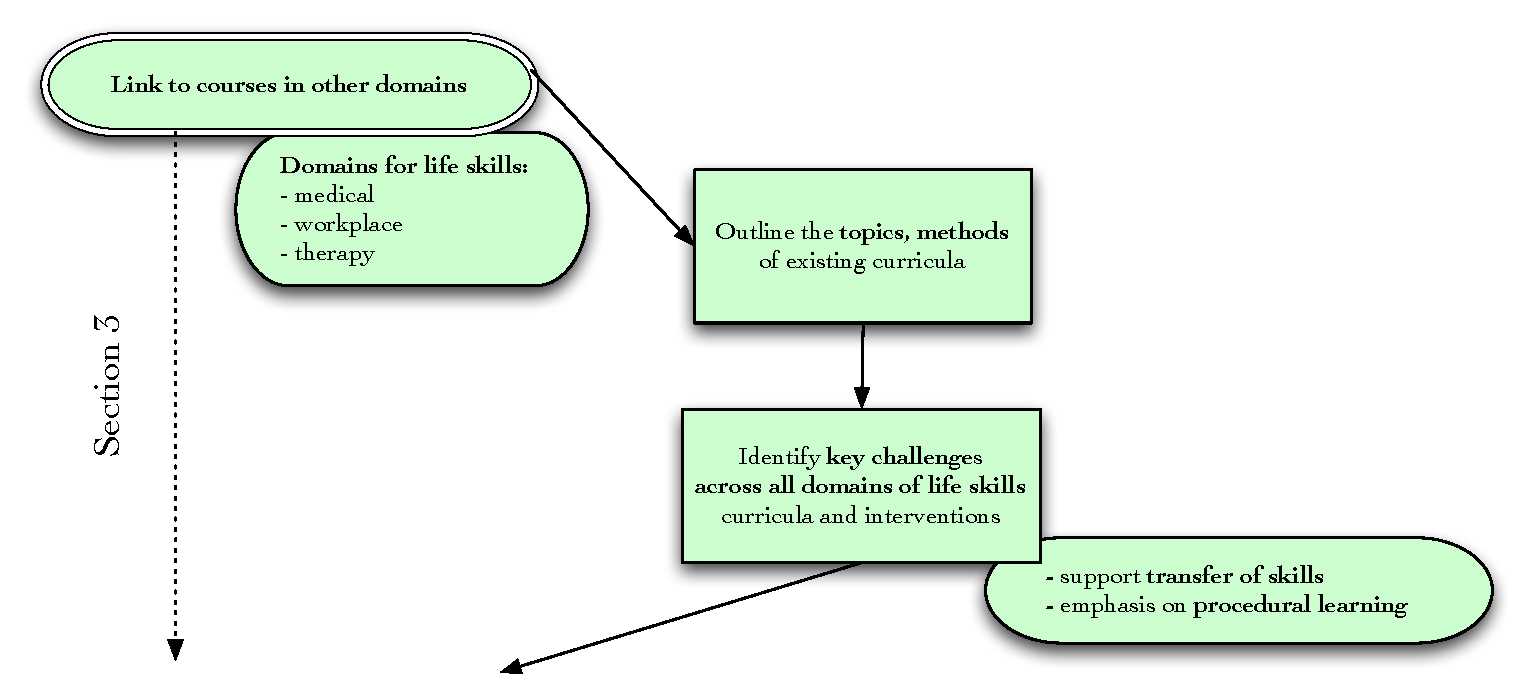
\includegraphics[scale=0.5]{imagess/JournalStructure3.pdf}
%       \caption{Overview of Section~\ref{sec:linkDomains}}
%       \label{fig:linkDomains}
%\end{figure}
  


%\vfill ~ \pagebreak
% \rephrase{These fit well to the 5 core values identified for SEL} 

% {{{ Therapy 
\paragraph{Talk-based therapeutic settings}
A crucial part of talk-based psychotherapy aims to support the development of social and life skills, often for clients  disadvantaged by cognitive or emotional deficits or going through difficult life situations at the time. % mainly for clients  with cognitive or other deficits.
%
The literature in this domain focuses on two main aspects. First is the psychotherapy itself, i.e., strategies to support learning and improvement on the part of the clients (e.g., \cite{Duncan2010}). The second aspect concerns the training and development of the skills needed by the therapists/counsellors themselves, with the emphasis on supporting the learning process for the trainees leading to sophisticated combinations of class based learning and practice with real clients (under supervision of an experienced therapist) \cite{Asay1999}. See \citeN{Coyle2007} for a succinct review of the most common psychotherapy schools and links to further resources; and \citeN{Hill2006} for a review existing literature on teaching counselling and psychotherapy students, showing significant positive effects of particular training methods.


\iffalse

\subsubsection*{Methods}  
The methods used to work with clients during the therapeutic process differ depending on the psychotherapy approach chosen by the therapist. These can range from very specific training situations and exercises such as exposure therapy in Cognitive Behavioural Therapies (CBT) or social skills training for people with autism, to unstructured exploration of personal experience in humanistic approaches.  See, e.g., \citeN{Coyle2007} for a succinct review of the most common psychotherapy schools and links to further resources; and \cite{Kientz2013} for an in-depth review of technologies developed to support autism therapy. 
%
Skills development for students and novice therapists builds on a mix of lectures on the theoretical background and how to put these into practice. This is done initially with peer students who role-play clients and share and discuss their (real) problems; later in the learning process this also involves real-clients, where the students lead the psychotherapy under close supervision of an experienced therapist. The emphasis on supervision is high, with the majority of schools/colleges requiring student therapists to enroll into psychotherapy for themselves while studying. 


\subsubsection*{Topics} 
In terms of supporting the client directly in the psychotherapy process, the topics differ substantially depending on the clients' issues or disorder, and personalisation is crucial. As such therapies can, for example, aim to help clients to achieve better self-awareness, to develop better  self-control, decision making processes, and interpersonal skills, and to help change deeply set negative thinking patterns.  %For a more specific example, clients with autism often have difficulties with basic social skills such as understanding emotional states of others or engaging/disengaging from interactions.  
% also examples from Coyle2011? -- depression, anxiety management
%\todo{add something on the effect of providing client feedback as a novel approach? }
%
Therapist training is most concerned with very detailed self-awareness on the part of the therapist, and mastering the techniques and approaches of the studied psychotherapy approach. The ability to empathise and fully listen to the clients is particularly emphasised as a key therapeutic skill. The aim of all these social and emotional skills is to help develop a good working relationship with clients, which is seen as one of the main aspects of successful psychotherapy \cite{Asay1999}.

\subsubsection*{Reviews}
Therapeutic settings have already generated considerable research within
HCI,  looking at using technology to extend and improve the psychotherapy process. The work so far focused mostly on autism related systems (e.g.,
\cite{Escobedo2012,Picard2009,Hayes2011,Porayska-Pomsta2011,Hong2012} and many others), and cognitive-behavioural therapies (e.g., \cite{Coyle2011,Matthews2011}). \citeN{Coyle2007} in particular gives an overview of the use of technology in psychotherapy, the potential for HCI involvement, and a solid introduction to most common psychotherapy styles.          
%
In addition, \citeN{Hill2006} review existing literature on teaching counselling and psychotherapy students, showing significant positive effects of particular training methods. The book edited by \citeN{Duncan2010} provides a detailed review of the factors common across various therapeutic approaches, including the large positive effect sizes of most therapies, and the key role of the therapeutic relationship. 

\fi


%\citeN{Vismara2010} reviews another for empathy as key for therapeutic process (maybe something from Marci + can use the Heart of therapy book)
%\item also reviews on the efficiency of therapy (maybe Coyle2007 has some?)
%\end{itemize}




%\Geraldine{ G: include as sub-section of clinical setting? also use some [pubsense seed paper refs] to motivate effectiveness of empathy in this relationship?}
%\begin{itemize}
%       \item .... not sure how much space this should get, given it has been already %addressed in earlier work. Although, I guess that this could also point to a slightly %different approaches than those used at the moment? 
%       \item Probably need to emphasise that each and every competency can be addressed, %depending on the therapy style/clients issues.
%       \item A short paragraph with link to David's review for specific work done in HCI. %Plus a few sentences linking the way how students become therapists, through again %role play, a lot of practice etc. Have a decent link for this \cite{Hill2007}, but %will ask Stef in Nottingham for others.
%       \item Also links to autism literature for additional examples?.
%\end{itemize}  
% }}}

% {{{ Medical settings
\paragraph{Clinical settings}

Social skills, such as communication skills and empathy, are increasingly recognised as core clinical skills in the medical community \cite{Rider2006,Barth2011,Makoul2007,Kalet2004}. Improvements in such skills have been shown to enhance patient satisfaction, increase adherence to therapy, and promote patient willingness to divulge sensitive information that may assist diagnosis as well as reduce the risk of subsequent litigations \cite{Stewart1995,Brown2008}. %As Brown \cite{Brown2008} puts it,  ``Over the last 20 years, the topic has raised from its status as a "nice to know" subject to that of a "need to know" skill set in modern medical education''. 
Most curricula focus on one of  three areas: (i) university courses for medical students \cite{Satterfield2007,Stepien2006}; (ii) general courses and support for practising medical personnel \cite{Rao2007}; and (iii) specialised courses for specific groups of medical personnel, such as in cancer care or end-of-life care, where specific skills related to empathy and communication are even more important (e.g., when giving bad news to patient) \cite{Barth2011}. Most of the courses are available for doctors, with courses also offered for nurses and other health professionals. Peer-reviewed evidence exists for the effectiveness of  many of the interventions in this domain for improving the targeted skills
(see the online appendix for more detail).
% also physios (who do a lot of motivational interviewing to help people develop rehab programs they can stick with etc)
% reference Yedidia2003 -- intervention for students 

\iffalse
\subsubsection*{Methods} A popular method in medical settings is the use of role play both with peers and using trained actors  \cite{Stepien2006,Stiefel2010,Kalet2004,Barth2011}, as well as facilitator or peer based feedback \cite{Rao2007}. 
\GeraldineFIX{G: \textbf{(G: on what?\ on the role plays, or is this another method ie not clear what 'followed by' refers to ... popularity or how role play is used)}}
Courses also include workshops, lectures, and discussions of case studies. Many courses that aim at general communication skills include role plays with scripted exchanges or examples to practise on. 
 \textbf{\GeraldineFIX{G: (G:\ how are these different to role plays??) P: These a specific sub-part of role plays (i.e., you can have other role plays without scripted exchange). I believe it is worth mentioning as such scripted (iu.e., fixed) exchanges can be readily supported by technology.}}


\subsubsection*{Topics} 
Curricula focus both on self-oriented emotional skills for medical personnel as well as a wide range of interpersonal interaction skills. 
%
Courses on self-oriented emotional skills include aspects such as personal reflection, self-awareness mindfulness, and stress management training \cite{Shapiro2000,Epstein1999,Satterfield2007}. This also incorporates the growing emphasis on the importance of teaching medical students and healthcare practitioners to manage their own well being, for example through teaching mindfulness techniques and lifestyle management \cite{Hassed2009}.
%
Courses on interpersonal skills aim to support generic patient-clinician interaction. The emphasis is on the ability to inquire for diagnosis related information and to clearly communicate test results and offer  treatment suggestions (e.g., see \cite{Kalet2004,Barth2011} for examples and review); related techniques, such as  motivational interviewing \cite{Miller2002},  focus on skilful framing of questions with the aim of empowering  clients to take responsibility for their own behaviours and decisions.  
\GeraldineFIXNEW{GF NOTE: Hettema is not a classic motivational interviewing ref - some Miller ref is better to use here eg Miller, W. R., \& Rollnick, S. (1991). Motivational interviewing: Preparing people for change. New York: Guilford Press. OR Rollnick, S., \& Miller, W.R. (1995). What is motivational interviewing? Behavioural and Cognitive Psychotherapy, 23, 325-334.}
%
 
Empathy is understood as another crucial component of successful and caring interactions between the patient and doctors, nurses and other health professionals. Empathy is particularly important in interactions communicating deeply emotional and life-changing information, e.g., in oncology, and to a lesser extent also in other general practice \cite{Barth2011}.
                For example, doctors often tend to ignore patients' emotions during difficult moments (e.g., having to communicate a critical diagnosis) and concentrate on the pragmatics, leading to negative consequences for treatment adherence and psychological functioning of patients. The training involves aspects such as sensitive responding to emotions from patients and improved understanding of the patients' psychosocial issues, concerns and needs as well as methods to do so while protecting the emotional well-being of the clinician or nurse. 


\GeraldineFIX{ G: say what technology how used in a sentence???}
\GeraldineFIX{ G: this doesn't seem to be empathy but about self awareness/regulation?  ... P: Is this a bit better? 
I'm drawing on the reviews and the concerns they use in this space -- in my reading it is also around objectification of the patient etc... where regulation is obviously important, but also as a part of being able to emphasise in these cases without burn-out etc. .. I think it might be too complex to go into details here (especially given what a tangled mess empathy as a concept is :)}
        %       \item Additional focus on specific communication skills  such as breaking bad news for oncologists and \todo{...}.

\subsubsection*{Reviews} \citeN{Rao2007} present a systematic review of interventions designed to enhance communication behaviours between patients and doctors, and \citeN{Barth2011} systematically review communication courses specialised for oncology personnel (e.g., doctors, nurses, social workers). Both  found statistically significant positive effects of skills training, such as improvements in patient-centered communication skills as well as higher ratings from the patients. Emotional skills training for medical students is reviewed by \cite{Satterfield2007} and shows positive effects of the interventions. \citeN{Pedersen2009} and \citeN{Stepien2006} review training courses that specifically aim to increase empathetic skills of students or practitioners. There have also been some successful initial studies
on including technology into the teaching process, e.g., \citeN{Tulsky2011}
shows the benefits of combining lectures with tailored video-recording of
the doctors' own interactions for later reflection.
\fi


% }}}

% {{{ Workplace and business relate
\paragraph{Workplace and business related settings}

A focus on emotional and social skills teaching also has a long history in the workplace, e.g.,  \cite{Bailey1983,Bailey1983a}, appearing under a wide range of labels such as interpersonal skills, soft-skills or, more recently, emotional intelligence and developmental workplace coaching. Social and emotional skills training is included as part of professional educational programmes such as for MBA and undergraduate business students; it is also offered as part of ongoing professional development in the workplace, e.g., many companies offer soft-skills courses or coaching to their executives and increasingly also to other staff. 
%
Academic literature shows positive effects of such training (such as improved leadership, team-building or self-management skills), but the existing evidence is not as strong as for SEL in education. Some of the reasons are that training programs have often been developed on a purely commercial basis and outside of the academic community  and detailed information about the content of the programs is often not available for intellectual property and/or competitive advantage reasons \cite{Walter2011,Clarke2006,Riggio2003}. 




\iffalse

\subsubsection*{Methods} The majority of courses follows similar strategies: role-play as a key approach to teaching the skills, together with discussion of fictional and real life cases, demonstrations and modeling. The emphasis is again placed on procedural learning and the opportunity to practise and embed skills so that they become automated. Time-frames differ from a few hours to multi-day courses, and to longer-term learning relationships (e.g., as in coaching). 

\subsubsection*{Topics} 
        A key focus is on developing aspects of emotional intelligence (EI), which can be defined as ``the ability to carry out accurate reasoning focused on emotions and the ability to use emotions and emotional knowledge to enhance thought'' \cite{Mayer2008}. Such training might, for example, develop communication and cooperation skills, as well as increase self-awareness of the employees. 
%        
        Specific leadership programs focussing on SEL skills in the workplace designed for executives are often aimed at relationship skills (such as conflict management and interviewing) and self-management (e.g., dealing with stress or time-planning and goal setting). Executives are often expected not only to learn these skills themselves, but also to be able to teach them to others later on. Coaching is often used as a way to help executives (and increasingly other employees) develop EI skills \cite{Bono2009}. It is inherently client-focussed, with the goals agreed depending on the situation, and emphasises accountability to the coaching relationship, honest feedback, supported reflection and accepting responsibility for own decisions. 

\GeraldineFIX{G: Not just for executives though in the workplace - this can sound like it is only for execs?    P: That's what the reviews I found focused on ... perhaps still mainly used for execs, as very expensive to roll-out more widely? Or perhaps not that much literature on it?}

\subsubsection*{Reviews}  \citeN{ArthurWinfred2003} provides a general overview of the effectiveness of training within organisations, including training of interpersonal skills, and discusses the effects of various training designs. Their meta analysis reveals medium to large positive effect sizes  ($d$ around $0.60$) for organisational training courses. \citeN{Mayer2008} gives a thorough review of the 'emotional intelligence' concept, including connections between emotional intelligence and better real-world performance.   \citeN{Feldman2005} and \citeN{Bono2009} summarise the practices and processes used in executive coaching by practitioners, and \citeN{Carey2011} provides a rigorous review of academic literature on work-place based coaching for leadership. \GeraldineFIX{G: ??? seeing you also mention coaching under the personal area?? ... P: But this review really does talk about work-place only, with particular focus on leadership}
\fi

% }}}

% {{{ Mindfulness
\paragraph{Everyday life skills}
Everyday life skills courses comprise a wide range of fragmented topics and methods. As such, we only briefly point to several illustrative examples where social and emotional intelligence skills are taught in, and for, everyday life settings. These are often framed as  various life skills courses  for the general population such as interventions supporting interpersonal skills (e.g., improving empathy for couples \cite{Long1999,Angera2006}) or interventions based on meditation, yoga, and more recently Mindfulness Based Stress Reduction \cite{Kabat-Zinn2003}, all aiming to support and improve personal well-being (e.g., \cite{Grossman2004,Marchand2012}).  %.  -- couldn't find any literature on courses that would not be for medically relevant population. My guess is that they exist (as per many such courses in the universities), but I have no reference to point to, yet. I also did not find an overarching review of mindfulness courses, closest available is \cite{Ludwig2008}. 
Moreover, the growth of life coaching (e.g., \cite{Green2006})  and consultation services, most commercially based, as well as the wide usage of self-help books, point to the increased recognition by people of the value of positive self-driven change and interpersonal and emotional regulation skills. 
%
Altogether, these examples draw out the large scope of everyday life skills learning, and the value people place on them.

% }}}



%}}}

% {{{ SECTION: Conclusions
\section{Conclusions}
\label{sec:conclusion}

This paper points to the potential of mutual cooperation between HCI and social and emotional skills learning (SEL), beginning with education, and benefiting both disciplines.
%
We outlined the key challenges for current SEL approaches, including the lack of support for transfer and 'embedding' of skills from the SEL lessons into students' interaction, encouraging parental involvement, as well as enhancing the support for development of reflective abilities and novel environments for practice. 
%
The review of existing HCI research shows there are strong indications that technology could help address many of these challenges. We drew on existing HCI work in a wide range of areas such as ubiquitous computing, emotional awareness and reflection, sensor-based tracking, social networks, design, and (serious) games. As such, HCI involvement in this space has the potential for strong, real-world impacts, especially given the wide (and ever increasing) penetration of SEL programs in our schools, workplaces and everyday life.  
%
We also highlighted how the focus on SEL provides new challenges for HCI, as well as a structure to further guide and support HCI research around social and emotional interactions -- both as a 'test-bed' to develop cutting-edge technology in, but also as a 'knowledge base' we can build and learn from as we shape this emerging research area for HCI. 
%
Overall, this paper suggests that social and emotional learning points to a novel, complex, intriguing research space, which has a high potential to enrich HCI research and practice.




%In doing so we have presented a set of structured concepts and characterisations of SEL to help frame an agenda for further research. We provide a summary of the topics, methods, and learning principles, and their associated challenges in SEL across the domains (Table~\ref{fig:SummaryResults}); we review HCI research relevant to the respective challenges (Table~\ref{fig:HCIsummary}) and outline the design space and opportunities for HCI  (Table~\ref{tab:session6summary}).



%



%




%We end by highlighting three selected aspects of SEL we personally find particularly interesting for immediate future work within HCI. These are (i) addressing the support for social and emotional learning in education of neuro-typical children (a domain with a long history, many curricula that are widely applied, but so far under-researched in HCI); (ii) the implications of supporting facilitated learning in SEL (and the differences in design settings it brings); and (iii) finding ways to mesh HCI research and technology support well with the curricula design (building on the long history of research there).
%       \todo{what this means for HCI}
%       \begin{itemize}
                % build on the special needs research to look at neurotypical groups
                % Focus on facilitated learning and the design implications it has -- in-class learning as an important settings to start from, and supporting out-of-class, ``in the wild'' learning as a way to address the key challenge.
%
%       \end{itemize}



%
%The distinction and characterisations we offered here are likely to be only an initial attempt to describe the nuances of the field.
%It is our hope that while the characterisations and distinctions suggested in this paper could be useful for immediate future work into this space, further research will elaborate on, clarify and extend, rather than reify, these.


%\todo{something feels wrong -- maybe not well balanced and/or missing the extent of research into autism (and other special interest groups?)}

% }}} 

\section*{Acknowledgements}
We are particularly grateful to David Coyle, Chris Frauenberger, Eva Ganglbauer, Brian Smith, and Anja Thieme for their thoughtful comments and suggestions on the earlier versions of this paper. Petr Slov\'{a}k has been supported in this work by the Austrian Academy Sciences under the DOC Fellowship. 



\bibliographystyle{acmsmall}
\bibliography{library}

\bigskip

\section*{Authors' statement}
This work is not, and has not been, submitted for a review in any other venue. No part of this work was previously published or has any direct relationship to our existing/submitted papers. 
\end{document}


